% !TeX root = main.tex
\documentclass{article}


%% Useful packages
\PassOptionsToPackage{usenames,dvipsnames,svgnames,table}{xcolor}
\usepackage[utf8]{inputenc}
\usepackage[a4paper,left=2cm,right=2cm,top=2cm,bottom=2cm]{geometry}
% \usepackage[a4paper,left=2cm,right=2cm,top=2cm,bottom=2cm,showframe]{geometry}
\usepackage{crop,graphicx,amsmath,array,color,amssymb,fancyhdr,lineno}
\usepackage{flushend,stfloats,amsthm,chngpage,times,lastpage,siunitx,chemformula}
\usepackage{calc,listings,color,wrapfig,tabularx,longtable,enumitem,rotating,booktabs}
% Minipage nonsense
\usepackage[most]{tcolorbox}
\usepackage[export]{adjustbox}
\usepackage{lineno}
\usepackage{tikz}
\usetikzlibrary{shapes,arrows,chains}
\usepackage{pstricks}
\usepackage{pgfplots}
\usepackage{pgfplotstable}
\usepackage{collcell}
\usepackage{pgf}
\usepackage{array}
\usepackage{subcaption}
\usepackage{etoolbox}
\usepackage{hyperref,bookmark}
\usepackage[backend=biber,style=ieee]{biblatex}
\addbibresource{Refs.bib}
\pgfplotsset{width=0.8\textwidth, compat=1.18}




%% Custom Commands
\definecolor{purple1}{RGB}{208, 180, 239}
\definecolor{purple2}{RGB}{190, 051, 218}
\definecolor{purple3}{RGB}{129, 000, 180}
\definecolor{purple4}{RGB}{087, 005, 139}

% Roman numerals \rom{2} = II
\makeatletter
\newcommand*{\rom}[1]{\expandafter\@slowromancap\romannumeral #1@}
\makeatother

% microLED
\newcommand{\uled}{$\mu$LED}
\newcommand{\uleds}{$\mu$LEDs}

% Units
\newcommand{\umm}   {\unit[per-mode=fraction]{\mu\meter\squared}}
\newcommand{\um}    {\unit[per-mode=fraction]{\micro\meter}}
\newcommand{\nm}    {\unit[per-mode=fraction]{\nano\meter}}
\newcommand{\mm}    {\unit[per-mode=fraction]{\milli\meter}}
\newcommand{\mA}    {\unit[per-mode=fraction]{\milli\ampere}}
\newcommand{\mV}    {\unit[per-mode=fraction]{\milli\volt}}
\newcommand{\mpa}   {\unit[per-mode=fraction]{\mega\pascal}}
\newcommand{\sqmm}  {\unit[per-mode=fraction]{\square\milli\meter}}
\newcommand{\junits}{\unit[per-mode=fraction]{\milli\ampere\per\square\milli\meter}}
\newcommand{\jufeet}{\unit[per-mode=fraction]{\ampere\per ft^2}}
\newcommand{\mmph}  {\unit[per-mode=fraction]{\mm\per\hour}}
\newcommand{\umpm}  {\unit[per-mode=fraction]{\um\per\minute}}
\newcommand{\dC}    {\unit[per-mode=fraction]{\degreeCelsius}}




\makeatletter
%% Minipage
% #1 Name
% #2 Indent
% #3 Beforeskip
% #4 Afterskip
% #5 Style
% #6 Heading
\newcommand*{\@mpstartsection}[6]{%
  \if@noskipsec \leavevmode \fi
  \par
  \@tempskipa #3\relax
  \@afterindenttrue
  \ifdim \@tempskipa <\z@
    \@tempskipa -\@tempskipa \@afterindentfalse
  \fi
  \if@nobreak
    \everypar{}%
  \else
    \addvspace\@tempskipa
  \fi
  \refstepcounter{cont@#1}% this counter is never reset, used for hyperref
  \stepcounter{#1}% counter used for display purposes
  \protected@edef\@currentlabel{% define how refs look
    \csname p@#1\endcsname \csname the#1\endcsname
  }%
  \protected@edef\@svsec{\@seccntformat{#1}\relax}%
  \begingroup
    #5{\@hangfrom{\hskip #2\relax\@svsec}#6\@@par}%
  \endgroup
  \par
  \vskip #4\relax
  % \@afterheading deals with penalities related to page breaking that aren't
  % needed inside a minipage, but it also honors the \if@afterindent switch,
  % therefore leave it here.
  \@afterheading
  \ignorespaces
}

\newcounter{mpsection}
\newcounter{mpsubsection}[mpsection]
\newcounter{cont@mpsection}
\newcounter{cont@mpsubsection}
\renewcommand\thempsection{\@arabic\c@mpsection}
\renewcommand\thempsubsection{\thempsection.\@arabic\c@mpsubsection}
\AtBeginEnvironment{minipage}{%
  \setcounter{mpsection}{0}%
}
\newcommand\mpsection{\@mpstartsection{mpsection}{\z@}{-3.5ex \@plus -1ex \@minus -.2ex}{2.3ex \@plus.2ex}{\normalfont\normalsize\bfseries}}
\newcommand\mpsubsection{\@mpstartsection{mpsubsection}{\z@}{-3.25ex \@plus -1ex \@minus -.2ex}{1.5ex \@plus .2ex}{\normalfont\normalsize\itshape}}


\makeatletter
\def\fillRGB#1#2#3{\pgfsys@color@rgb@fill{#1}{#2}{#3}}
\makeatother
\definecolor{purple4}{RGB}{087, 005, 139}
%======================================
% Color set related!
\definecolor{high}{HTML}{57058B}  % the color for the highest number in your data set
\definecolor{low}{HTML}{FFFFFF}  % the color for the lowest number in your data set
\newcommand*{\opacity}{70}% here you can change the opacity of the background color!
%======================================
% Data set related!
\newcommand*{\minval}{2.61}% define the minimum value on your data set
\newcommand*{\maxval}{18.1}% define the maximum value in your data set!

%======================================
% gradient function!
\newcommand{\gradient}[1]{
    % The values are calculated linearly between \minval and \maxval
    \ifdimcomp{#1pt}{>}{\maxval pt}{#1}{
        \ifdimcomp{#1pt}{<}{\minval pt}{#1}{
            \pgfmathparse{int(round(100*(#1/(\maxval-\minval))-(\minval*(100/(\maxval-\minval)))))}
            \xdef\tempa{\pgfmathresult}
            \cellcolor{high!\tempa!low!\opacity} #1
    }}
}
\newcommand{\grd}[1]{\gradient{#1} }
%======================================
% gradient function single cell!
\newcommand{\gradientcell}[6]{
    % The values are calculated linearly between \minval and \maxval
    \ifdimcomp{#1pt}{>}{#3 pt}{#1}{
        \ifdimcomp{#1pt}{<}{#2 pt}{#1}{
            \pgfmathparse{int(round(100*(#1/(#3-#2))-(\minval*(100/(#3-#2)))))}
            \xdef\tempa{\pgfmathresult}
            \cellcolor{#5!\tempa!#4!#6} #1
    }}
}



%%%%%%%%%%%%   Header and Footer  %%%%%%%%%%%%%
\pagestyle{fancy}
\fancypagestyle{plain}{%
  \renewcommand{\headrulewidth}{0pt}%
  \fancyhf{}%
}

\title{%
  Advanced Packaging for \uleds \ using Indium Electroplating \\
  \large In Fulfillment of ECE 499 Course Requirement}
\author{Kunal Chandan}

\begin{document}
\begin{titlepage}

\newcommand{\HRule}{\rule{\linewidth}{0.5mm}} % Defines a new command for the horizontal lines, change thickness here

%----------------------------------------------------------------------------------------
%	LOGO SECTION
%----------------------------------------------------------------------------------------
\center

\includegraphics[width=10cm]{Title/UoW2.png}\\[1cm] % Include a department/university logo - this will require the graphicx package
 
%----------------------------------------------------------------------------------------

\center % Center everything on the page

%----------------------------------------------------------------------------------------
%	HEADING SECTIONS
%----------------------------------------------------------------------------------------

\textsc{\LARGE University of Waterloo }\\[1.5cm] % Name of your university/college
\textsc{\Large Electrical \& Computer Engineering }\\[0.5cm] % Department Name
\textsc{\large ECE 499 Engineering Project}\\[0.5cm] % Course Title

%----------------------------------------------------------------------------------------
%	TITLE SECTION
%----------------------------------------------------------------------------------------
\makeatletter
\HRule \\[0.4cm]
{ \huge \bfseries \@title}\\[0.4cm] % Title of your document
\HRule \\[1.5cm]
 
%----------------------------------------------------------------------------------------
%	AUTHOR SECTION
%----------------------------------------------------------------------------------------

\begin{minipage}{0.4\textwidth}
\begin{flushleft} \large
\emph{Author:}\\
\@author % Your name
\\[1.2em]
\emph{ID No:}\\
20778788 \\[1.2em]
\end{flushleft}
\end{minipage}
~
\begin{minipage}{0.4\textwidth}
\begin{flushright} \large
\emph{Project Supervisor:} \\
 William Wong \\[1.2em] % Supervisor's Name
\emph{ECE 499 Course Coordinator:} \\
Mark Crowley % second marker's name
\end{flushright}
\end{minipage}\\[2cm]
\makeatother

% If you don't want a supervisor, uncomment the two lines below and remove the section above
%\Large \emph{Author:}\\
%John \textsc{Smith}\\[3cm] % Your name

%----------------------------------------------------------------------------------------
%	DATE SECTION
%----------------------------------------------------------------------------------------

{\large \today}\\[2cm] % Date, change the \today to a set date if you want to be precise

\vfill % Fill the rest of the page with whitespace

\end{titlepage}


\fancyhf{}
\fancyhead[L]{Kunal Chandan}
\fancyhead[R]{}
\fancyfoot[R]{ \bf\thepage\ \rm }%
\pagenumbering{gobble}


\newpage
\section*{Abstract}
Micro LEDs (\uled s) are an exciting, new technology that hold the potential to improve upon the capabilities of the incumbent display technologies of liquid crystal displays (LCDs) and organic light emitting diodes (OLEDs). Researchers and industry leaders deem \uled s capable of significant advantages in display technologies particularly with key performance metrics in contrast, colour gamut, pixel response timings, display lifetime, and power consumption.
Currently there are a variety of technical challenges in fabrication to making the dream of \uled \ displays a reality. During this research project I aim to assist in developing a process for packaging \uled  displays onto an addressable backplane.
To achieve this we use electroplated indium to create a mechanical and electrical connection between the \uled s and thin-film-transistor (TFT) backplane.


\newpage
\section*{Acknowledgements}
I would like to thank Prof. William Wong for allowing me to participate in his research lab and providing funding for the entire project, Pranav Gavirneni for being a supportive mentor through the entire research project.

\newpage
\tableofcontents
\listoffigures
\listoftables

\chapter*{Nomenclature}
\begin{table}[h!]
    \centering
\begin{tabular}{|p{2.5cm}|p{8cm}|p{2.5cm}|}
    \hline
    Symbol      & Definition        & Unit \\
    \hline
    \hline
    $A$         & Area              & [\unit{\square\milli\meter}] \\
    $I$         & Current           & [\unit{\ampere}] \\
    $J$         & Current Density   & [\junits] \\
    $V$         & Voltage           & [\unit{\milli\volt}] \\
    $R$         & Resistance        & [\unit{\ohm}] \\
    \hline
    \hline
\end{tabular}
\caption{Nomenclature Table}
\end{table}
\pagenumbering{arabic}
\setcounter{page}{1}
\section{Introduction}

LEDs are exceptionally efficient when compared to legacy lighting technologies like arc, incandescent, fluorescent lighting, and others. The advantages inherent to the technology have allowed LEDs to enter a variety of light applications like automotive, general lighting, and display backlighting and many other use-cases. \cite{uLED_review}
Conventional inorganic LEDs have MESA dimensions generally greater than $(300\times 300) \unit{\micro\meter\squared}$, however \uled s target an area below $(100\times 100) \unit{\micro\meter\squared}$ to $1 \unit{\micro\meter\squared}$ \cite{parbrook2021micro}

One of the earliest claims to the discoveries of the LED was by Oleg Losev in the 1920s, the work was generally ignored and the conjectured theory for the operation was incorrect, the subsequent research also focused on SiC and \rom{2}-\rom{4} semiconductors. This era of research was generally impractical and did not produce sufficient light. However, with the arrival of \rom{3}-\rom{5} semiconductors like GaAs, GaSb, InP, and SiGe there was significant progress in luminosity although sadly this was all within the infrared spectrum. 
Visible LEDs would emerge as research in the area quickened, the technology was based on GaAsP epitaxy over GaAs substrates. This would bring forth the advent of commercializable LEDs that would now be seen everywhere. Eventually efficiency and luminosity would surpass that of traditional lighting solutions like filament based tungsten and bring us to where we are today with LEDs being used in nearly all lighting and display applications.




\subsection{Motivation for \uled s as a Technology}
LCDs and OLEDs currently dominate the display market, each technology comes with its trade-offs and current innovations with quantum dots and fully addressable back-lit mini-LED panels aim to address some of the shortcomings concerning contrast, colour accuracy, power consumption, brightness, lifetime, and response times.

\uled s aim to address many of these concerns as well, by offering a number of advantages over traditional LCD and OLED displays. The biggest advantage \uled s would provide over LCDs is the power effeciency where LCDs suffer from high power loss due to the multiple diffuser and filtering layers required to compose a screen (CITE AND REWORD). A commonly cited number is that LCDs loose nearly 70-90\% of the flux introduced by the backlight to the various polarizing layers that comprise the display. In contrast as \uled  displays would be entirely emissive, none of the light would be lost to the conventional filtering layers. (IS THIS EVEN TRUE, IS LIGHT LOST TO PHOSPHOR LAYERS?)


\subsection{Hurdles in \uled Technology}

IDENTIFY COMMON HURDLES IN MICRO LED TECHNOLOGY

SHOW WHICH OF THESE PROBLEMS WE ARE AIMING TO FIX OR SOLVE FOR


\subsection{Motivation for Indium as a Diebonding Material}

EASE OF INDIUM AS AN ELECTROPLATING MATERIAL

LOW MELTING POINT

SOFTNESS OF MATERIAL/DUCTILITY

LOW LIKELYHOOD OF SURFACE OXIDES

EASE OF WETTING TO SURFACE

\newpage
\section{Indium Electroplating}

\subsection{Introduction}
There are a variety of methods for indium electroplating, while I did not select the electroplating process there are a variety of methods available that are commonly used in industry. The largest differences tend to be in what comprises the solution and the operating temperatures.

\subsection{Process}
The indium electroplating process is based on a now industry standard process that is known to yield good results while requiring a minimum of process optimization.

CITE THE INDIUM CORPORATION AND THE ADDITIVES IN THEIR ELECTROPLATING SOLUTION

IDENTIFY BENEFITS OF EACH CHEMICAL IN THE THING? IF POSSIBLE?

Adapting the indium electroplating process to the E3-3139 and the resources available there, the process is in \hyperref[sec:SOP]{Appendix A}.

The process used there allows us to electroplate indium onto the substrate that is Chrome-Gold on Sapphire. Both chromium and gold are excellent materials for indium to easily electroplate onto.
% TODO PROVIDE CITATION

\newpage

\subsection{Existing Setup Description}

In summary the process has us prepare the sample with acids before placing into the plating solution. Then the sample holder and sample are submerged in the plating solution and the current source is applied. However, due to cost constraints a voltage source was obtained to perform in place of a current source.

\begin{wrapfigure}{L}{0.25\textwidth}
    \centering
    \includegraphics[width=0.25\textwidth, angle=90]{Main/Ch1/Aligator_clip.jpeg}
    \caption{\raggedright Image of the flat mouth alligator clip used to clamp onto the sample}
\end{wrapfigure}

A current source would have been preferred over a voltage source due to several reasons. Since electroplating is a process where metal ions are deposited on a substrate through the use of an electric current. The amount of metal deposited is directly proportional to the amount of electric charge that flows through the system, which means that controlling the current is crucial for controlling the thickness and quality of the plated layer.

With a current source, the current can be precisely controlled and maintained at a constant level, which results in consistent and uniform plating as a function of time. On the other hand, a voltage source may not provide a consistent current, as the resistance of the plating solution can vary due to factors such as temperature or impurities, leading to poor plating results.


\begin{wrapfigure}{R}{0.25\textwidth}
    \centering
    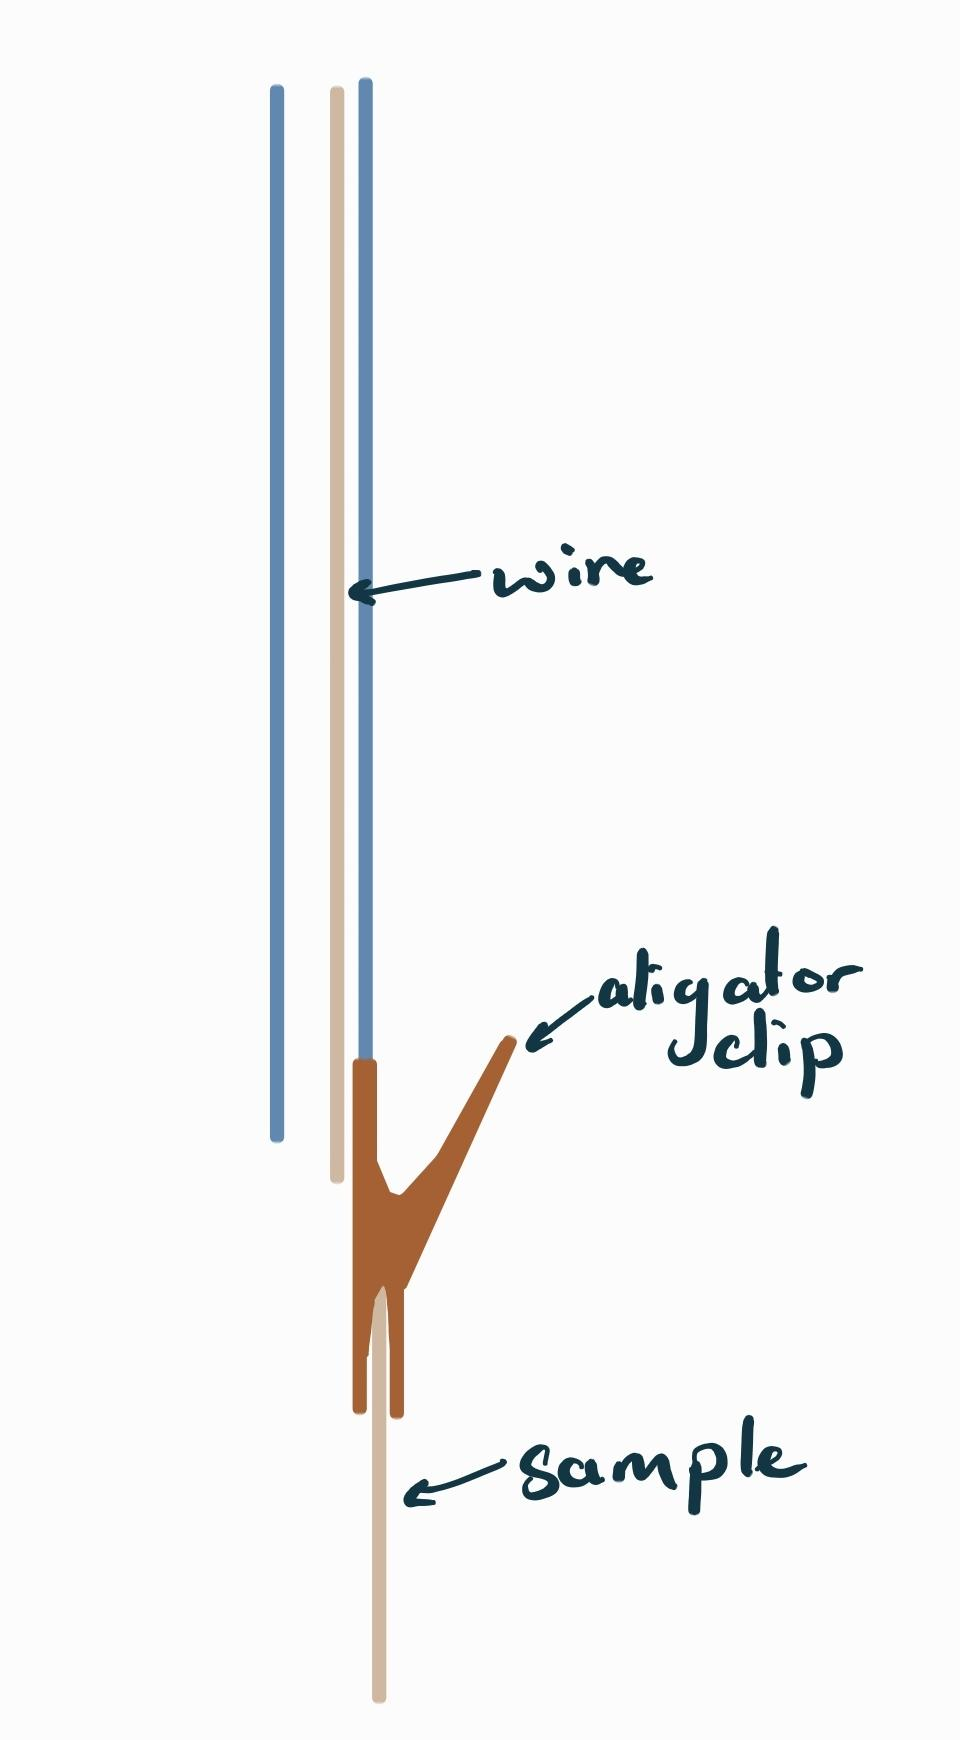
\includegraphics[width=0.25\textwidth]{Main/Ch1/Current Sample holder.png}
    \caption{Line drawing of the alligator clip and sample }
\end{wrapfigure}

Another advantage of using a current source is that it allows for better control over the plating process and reduces the risk of over-plating or under-plating. With a voltage source, the voltage applied to the system can cause the plating rate to fluctuate, which can result in uneven thickness or even damage to the substrate. In contrast, a current source ensures a constant and controlled deposition rate, which minimizes the risk of defects or damage to the substrate.

Using a voltage source with an ammeter can be equivalent to a current source in certain situations. This is because the voltage applied to a circuit is directly proportional to the current flowing through it. By measuring the current in the circuit using an ammeter, the current can be controlled by adjusting the voltage. In this way, the voltage source with an ammeter can effectively act as a current source.


\begin{wrapfigure}{L}{0.25\textwidth}
    \centering
    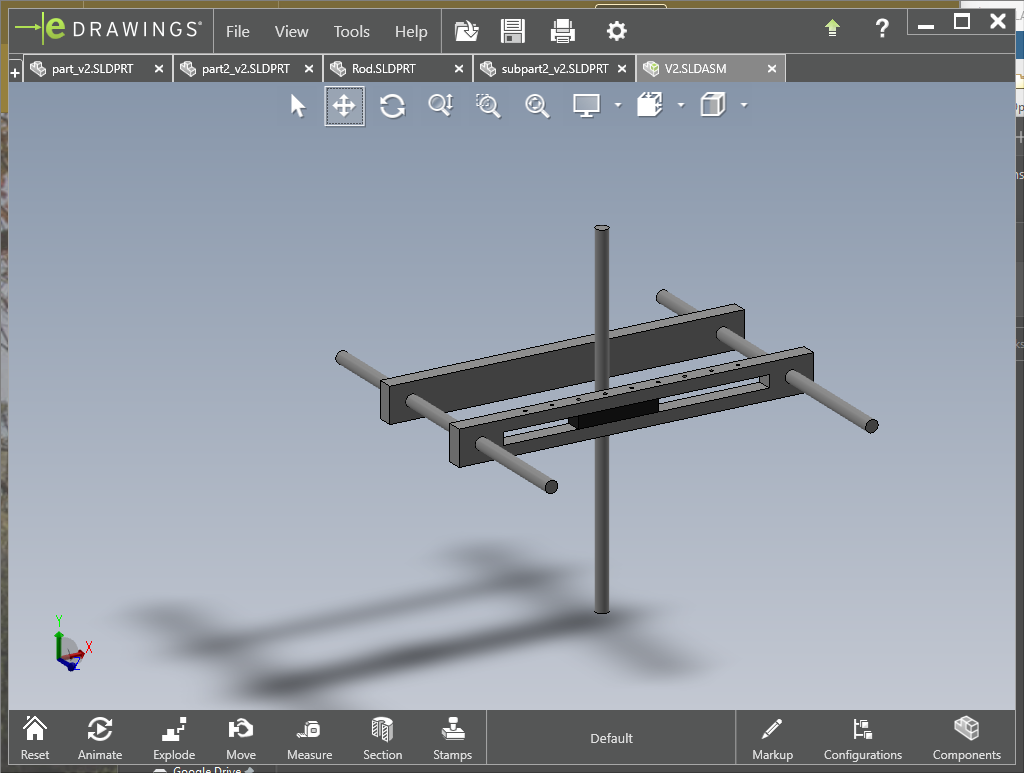
\includegraphics[width=0.25\textwidth]{Main/Ch1/Sample_holder.png}
    \caption{3D Rendering of the sample holder}
\end{wrapfigure}

The sample holder consists of two plastic blocks that are held together by two steel bars. Thumbscrews are used to lock the relative position of the plastic pieces in place while the assembly 'floats'  on the lip of the beaker the sample is submerged into. One of the two plastic pieces has a stopper that helps constrain the position of the assembly on the beaker while the other plastic piece holds the glass rod and alligator clip.

The glass rod is attached to the plastic piece and has the alligator clip on it. The clip and corresponding cathode holder are wrapped in a PTFE sleeve that helps minimize stray electric fields and electroplating onto the cathode wire.



\subsection{Physical Problems with the setup}

% TODO Replace with SI units instead of mA ...
% TODO Replace derivative with derivative library maybe?
The existing setup came with an analog voltage supply that was only able to provide analog control of the voltage based on two knobs (a fine and coarse). This control was only fine enough to $\pm 10mV$ where the derivative of the current with respect to voltage in the relevant regime was $\frac{d mA}{d mV} = \frac{0.3 mA}{1 mV}$.
This meant there was poor resolution on the current control with the previous power-supply with a current resolution of $\pm 3 mA$ which would be an insufficient resolution for the small area that was being plated.

I replaced the existing voltage supply with a Tektronics function generator as it provided an appropriate resolution and dynamic range for such the task.
The function generator would allow for pulsed plating as recommended by the indium corporation \cite{indiumCorpGrainStructure}

\subsection{Experimental Issues - Deviation from Theory}

According to the Indium corporation docs, the recommended electroplating current density for plating is \dots
Converting to SI units from ASME units we see that this yields a plating current of \dots. However, in this analysis we have only considered the active plating area of the sample, and we have failed to consider the plating area of the exposed alligator clip that holds the sample.

The extra exposed area guarantees an incorrect characterization of the plating growth proportional to the exposed area for the indium bumps. We can show this simply from the following

\begin{equation}\tag{A}
    \begin{split}
        V &\doteq I R \\
        I_{Plating} &\doteq J_{Plating} \times A_{Plating} \\
        R_{Total} &\doteq R_{Anode} + R_{Plating Solution} + R_{Cathode} + R_{Wires} \\
        V_{Plating} &\doteq \text{Variable to satisfy plating current}
    \end{split}
\end{equation}

From the datasheets from Indium Corporation \cite{indiumCorpPlating} we see that the recommended plating current density.

$$
    J_{Plating} = 10-100 \unit{\ampere\per ft^2}
$$

Or in more elegant units:

\begin{equation}\notag
    \begin{split}
        J_{Plating} &\approx 1.1\times10^{-7}-1.1\times10^{-6}
        \unit{\milli\ampere\per\square\micro\meter} \\
        &= 0.11-1.1 \junits
    \end{split}
\end{equation}


We can then solve for the plating current based on the exposed area given by the GDS file of the sample.


\begin{wrapfigure}{R}{0.25\textwidth}
    \centering
    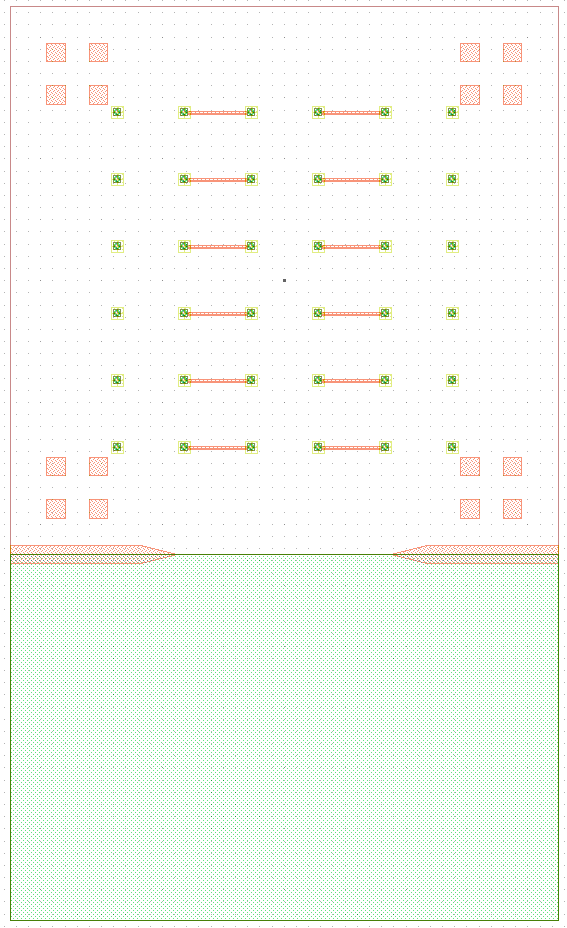
\includegraphics[width=0.25\textwidth]{Main/Ch1/GDS_V1.png}
    \caption{GDS image of the layout. Indium is in green bumps have a diameter of 40 $\unit{\micro\meter}$}
\end{wrapfigure}


The exposed area is thus:

\begin{equation}\notag
    \begin{split}
        A_{Plating} &= \pi (20 \um)^2 + (4.5 \mm \times 3 \mm) \\
        &\approx 13.5 \sqmm
    \end{split}
\end{equation}

Thus, the plating current for a current density of $20\unit{\ampere\per ft^2}$ or $0.2153 \junits$ is:

\begin{equation}\notag
    \begin{split}
        I_{Plating} &\doteq J_{Plating} \times A_{Plating} \\
        I_{Plating} &= (0.2153 \junits) \times (13.5 \sqmm)
    \end{split}
\end{equation}


HERE I WANT TO IDENTIFY THE PLATING GROWTH PER SECOND AS A FUNCTION OF THE PLATING AREA

DESIGN OF ALLIGATOR CLIP WAS MESSING WITH OUR RESULTS

ACCOUNTING FOR THE AREA OF THE ALLIGATOR CLOP

DERIVING THE AREA OF THE ALLIGATOR CLOP BASED ON EXPECTED PLATING GROWTH RATE



\subsection{Development of a Repeatable Process}

TO DEVELOP A REPEATABLE PROCESS PICKING A DISTANCE AND ENSURING ALIGNMENT

SELECTING A BETTER VOLTAGE SOURCE/CURRENT SOURCE MILLIVOLT CONTROL, RESOLUTION OF 0.02mA per mill Volt


\newpage
\section{Phase 1 - Uniform Bonding}

\subsection{Process}
The process in this section will aim to first characterize the spread of indium over the surface \ref{sec:indiumSpread} of the `LED' and `backplane' (`BP') substrates
\footnote{The LED and backplane are in quotes as these are not actual LEDs or backplanes with transistors, but instead are mock samples with similar physical characteristics.
Those characteristics being the sample size and the $\ch{In}-\ch{Au}$ coating on the samples.
Differences arise from the lack of a MESA structure that will be seen in the successive chapter
\ref{sec:BondingToLEDS}}
and secondly validate uniform bonding over the surface of the sample \ref{sec:uniformBond}.

The process that will be used to explore this is the following.
\begin{enumerate}
    \item Electroplate indium onto a `BP'
    \item Remove photoresist from sample with Acetone then IPA rinse or RemoverPG
    \item Do surface activation of LED and BP using the plasma-cleaner
    \item Place BP face up on diebonder, and LED face down on diebonder
    \item Using Pick-And-Place function on diebonder, pick the LED and place on the BP using the specified bonding pressure and heat recipe
\end{enumerate}


\subsection{Characterization of Indium Bonding Spread}
\label{sec:indiumSpread}
After a repeatable electroplating process for indium was developed, the next step was to investigate how the indium would spread once die-bonded. The spreading behaviour of indium is critical because it can impact the performance of the semiconductor device. Specifically, the spreading of indium can affect the heat dissipation and the electrical contact between the die and the substrate. Understanding this behaviour is essential for optimizing the performance of the device.
This knowledge can then be used to inform the design and manufacture of semiconductor devices, improving their reliability and performance.
Diebonding is the process of placing a semiconductor chip onto a substrate or package, and eutectic bonding is a common diebonding technique. Understanding the behaviour of indium during eutectic bonding is crucial for ensuring the reliability and performance of the final device.

\begin{figure}
    \centering
    \tiny
    \begin{tikzpicture}
        % define cell size
        \def\cSz{0.4cm}
        \def\N{12}

        % draw table border
        \draw (0,0) rectangle (\N*\cSz,\N*\cSz);

        \foreach \x in {1,2,3,4,5,6,7,8,9,10,11} {
            % draw horizontal lines
            \draw (0,\x*\cSz) -- (\N*\cSz,\x*\cSz);
            % draw vertical lines
            \draw (\x*\cSz,0) -- (\x*\cSz,\N*\cSz);
        }
        % add cell contents
        \draw[fill=purple4!28.3, draw] (0.0 * \cSz, 0.0 * \cSz) rectangle (1.0 * \cSz, 1.0 * \cSz);
\node at (0.5 * \cSz, 0.5 * \cSz)  { 4.80 };
\draw[fill=purple4!32.2, draw] (0.0 * \cSz, 2.0 * \cSz) rectangle (1.0 * \cSz, 3.0 * \cSz);
\node at (0.5 * \cSz, 2.5 * \cSz)  { 5.22 };
\draw[fill=purple4!19.6, draw] (0.0 * \cSz, 5.0 * \cSz) rectangle (1.0 * \cSz, 6.0 * \cSz);
\node at (0.5 * \cSz, 5.5 * \cSz)  { 3.98 };
\draw[fill=purple4!20.4, draw] (0.0 * \cSz, 6.0 * \cSz) rectangle (1.0 * \cSz, 7.0 * \cSz);
\node at (0.5 * \cSz, 6.5 * \cSz)  { 4.05 };
\draw[fill=purple4!33.1, draw] (0.0 * \cSz, 9.0 * \cSz) rectangle (1.0 * \cSz, 10.0 * \cSz);
\node at (0.5 * \cSz, 9.5 * \cSz)  { 5.32 };
\draw[fill=purple4!33.2, draw] (0.0 * \cSz, 11.0 * \cSz) rectangle (1.0 * \cSz, 12.0 * \cSz);
\node at (0.5 * \cSz, 11.5 * \cSz)  { 5.33     };
\draw[fill=purple4!11.3, draw] (2.0 * \cSz, 5.0 * \cSz) rectangle (3.0 * \cSz, 6.0 * \cSz);
\node at (2.5 * \cSz, 5.5 * \cSz)  { 3.33 };
\draw[fill=purple4!28.8, draw] (2.0 * \cSz, 6.0 * \cSz) rectangle (3.0 * \cSz, 7.0 * \cSz);
\node at (2.5 * \cSz, 6.5 * \cSz)  { 4.85 };
\draw[fill=purple4!0.0, draw] (3.0 * \cSz, 0.0 * \cSz) rectangle (4.0 * \cSz, 1.0 * \cSz);
\node at (3.5 * \cSz, 0.5 * \cSz)  { 2.61 };
\draw[fill=purple4!9.2, draw] (3.0 * \cSz, 3.0 * \cSz) rectangle (4.0 * \cSz, 4.0 * \cSz);
\node at (3.5 * \cSz, 3.5 * \cSz)  { 3.18 };
\draw[fill=purple4!28.4, draw] (3.0 * \cSz, 8.0 * \cSz) rectangle (4.0 * \cSz, 9.0 * \cSz);
\node at (3.5 * \cSz, 8.5 * \cSz)  { 4.81 };
\draw[fill=purple4!33.8, draw] (3.0 * \cSz, 11.0 * \cSz) rectangle (4.0 * \cSz, 12.0 * \cSz);
\node at (3.5 * \cSz, 11.5 * \cSz)  { 5.40     };
\draw[fill=purple4!6.8, draw] (5.0 * \cSz, 0.0 * \cSz) rectangle (6.0 * \cSz, 1.0 * \cSz);
\node at (5.5 * \cSz, 0.5 * \cSz)  { 3.02 };
\draw[fill=purple4!8.1, draw] (5.0 * \cSz, 2.0 * \cSz) rectangle (6.0 * \cSz, 3.0 * \cSz);
\node at (5.5 * \cSz, 2.5 * \cSz)  { 3.11 };
\draw[fill=purple4!18.4, draw] (5.0 * \cSz, 5.0 * \cSz) rectangle (6.0 * \cSz, 6.0 * \cSz);
\node at (5.5 * \cSz, 5.5 * \cSz)  { 3.88 };
\draw[fill=purple4!32.8, draw] (5.0 * \cSz, 6.0 * \cSz) rectangle (6.0 * \cSz, 7.0 * \cSz);
\node at (5.5 * \cSz, 6.5 * \cSz)  { 5.29 };
\draw[fill=purple4!17.2, draw] (5.0 * \cSz, 9.0 * \cSz) rectangle (6.0 * \cSz, 10.0 * \cSz);
\node at (5.5 * \cSz, 9.5 * \cSz)  { 3.78 };
\draw[fill=purple4!18.4, draw] (5.0 * \cSz, 11.0 * \cSz) rectangle (6.0 * \cSz, 12.0 * \cSz);
\node at (5.5 * \cSz, 11.5 * \cSz)  { 3.88     };
\draw[fill=purple4!42.8, draw] (6.0 * \cSz, 0.0 * \cSz) rectangle (7.0 * \cSz, 1.0 * \cSz);
\node at (6.5 * \cSz, 0.5 * \cSz)  { 6.55 };
\draw[fill=purple4!70.9, draw] (6.0 * \cSz, 2.0 * \cSz) rectangle (7.0 * \cSz, 3.0 * \cSz);
\node at (6.5 * \cSz, 2.5 * \cSz)  { 12.0 };
\draw[fill=purple4!90.0, draw] (6.0 * \cSz, 5.0 * \cSz) rectangle (7.0 * \cSz, 6.0 * \cSz);
\node at (6.5 * \cSz, 5.5 * \cSz)  { 18.1 };
\draw[fill=purple4!29.7, draw] (6.0 * \cSz, 6.0 * \cSz) rectangle (7.0 * \cSz, 7.0 * \cSz);
\node at (6.5 * \cSz, 6.5 * \cSz)  { 4.94 };
\draw[fill=purple4!25.8, draw] (6.0 * \cSz, 9.0 * \cSz) rectangle (7.0 * \cSz, 10.0 * \cSz);
\node at (6.5 * \cSz, 9.5 * \cSz)  { 4.55 };
\draw[fill=purple4!30.3, draw] (6.0 * \cSz, 11.0 * \cSz) rectangle (7.0 * \cSz, 12.0 * \cSz);
\node at (6.5 * \cSz, 11.5 * \cSz)  { 5.01     };
\draw[fill=purple4!39.8, draw] (8.0 * \cSz, 0.0 * \cSz) rectangle (9.0 * \cSz, 1.0 * \cSz);
\node at (8.5 * \cSz, 0.5 * \cSz)  { 6.15 };
\draw[fill=purple4!40.8, draw] (8.0 * \cSz, 3.0 * \cSz) rectangle (9.0 * \cSz, 4.0 * \cSz);
\node at (8.5 * \cSz, 3.5 * \cSz)  { 6.28 };
\draw[fill=purple4!56.6, draw] (8.0 * \cSz, 5.0 * \cSz) rectangle (9.0 * \cSz, 6.0 * \cSz);
\node at (8.5 * \cSz, 5.5 * \cSz)  { 8.82 };
\draw[fill=purple4!39.0, draw] (8.0 * \cSz, 11.0 * \cSz) rectangle (9.0 * \cSz, 12.0 * \cSz);
\node at (8.5 * \cSz, 11.5 * \cSz)  { 6.04     };
\draw[fill=purple4!29.7, draw] (9.0 * \cSz, 6.0 * \cSz) rectangle (10.0 * \cSz, 7.0 * \cSz);
\node at (9.5 * \cSz, 6.5 * \cSz)  { 4.95 };
\draw[fill=purple4!27.0, draw] (9.0 * \cSz, 9.0 * \cSz) rectangle (10.0 * \cSz, 10.0 * \cSz);
\node at (9.5 * \cSz, 9.5 * \cSz)  { 4.67 };
\draw[fill=purple4!40.3, draw] (11.0 * \cSz, 0.0 * \cSz) rectangle (12.0 * \cSz, 1.0 * \cSz);
\node at (11.5 * \cSz, 0.5 * \cSz)  { 6.21 };
\draw[fill=purple4!67.3, draw] (11.0 * \cSz, 2.0 * \cSz) rectangle (12.0 * \cSz, 3.0 * \cSz);
\node at (11.5 * \cSz, 2.5 * \cSz)  { 11.1 };
\draw[fill=purple4!55.3, draw] (11.0 * \cSz, 5.0 * \cSz) rectangle (12.0 * \cSz, 6.0 * \cSz);
\node at (11.5 * \cSz, 5.5 * \cSz)  { 8.57 };
\draw[fill=purple4!30.9, draw] (11.0 * \cSz, 6.0 * \cSz) rectangle (12.0 * \cSz, 7.0 * \cSz);
\node at (11.5 * \cSz, 6.5 * \cSz)  { 5.08 };
\draw[fill=purple4!35.0, draw] (11.0 * \cSz, 9.0 * \cSz) rectangle (12.0 * \cSz, 10.0 * \cSz);
\node at (11.5 * \cSz, 9.5 * \cSz)  { 5.54 };
\draw[fill=purple4!38.6, draw] (11.0 * \cSz, 11.0 * \cSz) rectangle (12.0 * \cSz, 12.0 * \cSz);
\node at (11.5 * \cSz, 11.5 * \cSz)  { 5.99     };


    \end{tikzpicture}
    \caption{Indium bump height map. Saturation of colour indicates relative thickness.}
    \label{fig:bumpHeightMap}
\end{figure}

\begin{figure}
    \centering
    \tiny
    \begin{tikzpicture}
        % define cell size
        \def\cSz{0.4cm}
        \def\N{12}

        % draw table border
        \draw (0,0) rectangle (\N*\cSz,\N*\cSz);

        \foreach \x in {1,2,3,4,5,6,7,8,9,10,11} {
            % draw horizontal lines
            \draw (0,\x*\cSz) -- (\N*\cSz,\x*\cSz);
            % draw vertical lines
            \draw (\x*\cSz,0) -- (\x*\cSz,\N*\cSz);
        }
        % add cell contents
        \draw[fill=purple4!16.0, draw] (0.0 * \cSz, 0.0 * \cSz) rectangle (1.0 * \cSz, 1.0 * \cSz);
\node at (0.5 * \cSz, 0.5 * \cSz)  { 16.4 };
\draw[fill=purple4!37.8, draw] (0.0 * \cSz, 2.0 * \cSz) rectangle (1.0 * \cSz, 3.0 * \cSz);
\node at (0.5 * \cSz, 2.5 * \cSz)  { 18.7 };
\draw[fill=purple4!17.0, draw] (0.0 * \cSz, 5.0 * \cSz) rectangle (1.0 * \cSz, 6.0 * \cSz);
\node at (0.5 * \cSz, 5.5 * \cSz)  { 16.5 };
\draw[fill=purple4!12.9, draw] (0.0 * \cSz, 6.0 * \cSz) rectangle (1.0 * \cSz, 7.0 * \cSz);
\node at (0.5 * \cSz, 6.5 * \cSz)  { 16.1 };
\draw[fill=purple4!17.0, draw] (0.0 * \cSz, 9.0 * \cSz) rectangle (1.0 * \cSz, 10.0 * \cSz);
\node at (0.5 * \cSz, 9.5 * \cSz)  { 16.5 };
\draw[fill=purple4!11.8, draw] (0.0 * \cSz, 11.0 * \cSz) rectangle (1.0 * \cSz, 12.0 * \cSz);
\node at (0.5 * \cSz, 11.5 * \cSz)  { 16.0     };
\draw[fill=purple4!12.9, draw] (2.0 * \cSz, 5.0 * \cSz) rectangle (3.0 * \cSz, 6.0 * \cSz);
\node at (2.5 * \cSz, 5.5 * \cSz)  { 16.1 };
\draw[fill=purple4!11.8, draw] (2.0 * \cSz, 6.0 * \cSz) rectangle (3.0 * \cSz, 7.0 * \cSz);
\node at (2.5 * \cSz, 6.5 * \cSz)  { 16.0 };
\draw[fill=purple4!22.9, draw] (3.0 * \cSz, 0.0 * \cSz) rectangle (4.0 * \cSz, 1.0 * \cSz);
\node at (3.5 * \cSz, 0.5 * \cSz)  { 17.1 };
\draw[fill=purple4!14.9, draw] (3.0 * \cSz, 3.0 * \cSz) rectangle (4.0 * \cSz, 4.0 * \cSz);
\node at (3.5 * \cSz, 3.5 * \cSz)  { 16.3 };
\draw[fill=purple4!5.5, draw] (3.0 * \cSz, 8.0 * \cSz) rectangle (4.0 * \cSz, 9.0 * \cSz);
\node at (3.5 * \cSz, 8.5 * \cSz)  { 15.4 };
\draw[fill=purple4!10.8, draw] (3.0 * \cSz, 11.0 * \cSz) rectangle (4.0 * \cSz, 12.0 * \cSz);
\node at (3.5 * \cSz, 11.5 * \cSz)  { 15.9     };
\draw[fill=purple4!21.9, draw] (5.0 * \cSz, 0.0 * \cSz) rectangle (6.0 * \cSz, 1.0 * \cSz);
\node at (5.5 * \cSz, 0.5 * \cSz)  { 17.0 };
\draw[fill=purple4!19.0, draw] (5.0 * \cSz, 2.0 * \cSz) rectangle (6.0 * \cSz, 3.0 * \cSz);
\node at (5.5 * \cSz, 2.5 * \cSz)  { 16.7 };
\draw[fill=purple4!7.6, draw] (5.0 * \cSz, 5.0 * \cSz) rectangle (6.0 * \cSz, 6.0 * \cSz);
\node at (5.5 * \cSz, 5.5 * \cSz)  { 15.6 };
\draw[fill=purple4!14.9, draw] (5.0 * \cSz, 6.0 * \cSz) rectangle (6.0 * \cSz, 7.0 * \cSz);
\node at (5.5 * \cSz, 6.5 * \cSz)  { 16.3 };
\draw[fill=purple4!5.5, draw] (5.0 * \cSz, 9.0 * \cSz) rectangle (6.0 * \cSz, 10.0 * \cSz);
\node at (5.5 * \cSz, 9.5 * \cSz)  { 15.4 };
\draw[fill=purple4!9.8, draw] (5.0 * \cSz, 11.0 * \cSz) rectangle (6.0 * \cSz, 12.0 * \cSz);
\node at (5.5 * \cSz, 11.5 * \cSz)  { 15.8     };
\draw[fill=purple4!0.0, draw] (6.0 * \cSz, 0.0 * \cSz) rectangle (7.0 * \cSz, 1.0 * \cSz);
\node at (6.5 * \cSz, 0.5 * \cSz)  { 14.9 };
\draw[fill=purple4!63.3, draw] (6.0 * \cSz, 2.0 * \cSz) rectangle (7.0 * \cSz, 3.0 * \cSz);
\node at (6.5 * \cSz, 2.5 * \cSz)  { 21.8 };
\draw[fill=purple4!90.0, draw] (6.0 * \cSz, 5.0 * \cSz) rectangle (7.0 * \cSz, 6.0 * \cSz);
\node at (6.5 * \cSz, 5.5 * \cSz)  { 25.6 };
\draw[fill=purple4!31.4, draw] (6.0 * \cSz, 6.0 * \cSz) rectangle (7.0 * \cSz, 7.0 * \cSz);
\node at (6.5 * \cSz, 6.5 * \cSz)  { 18.0 };
\draw[fill=purple4!44.7, draw] (6.0 * \cSz, 9.0 * \cSz) rectangle (7.0 * \cSz, 10.0 * \cSz);
\node at (6.5 * \cSz, 9.5 * \cSz)  { 19.5 };
\draw[fill=purple4!27.7, draw] (6.0 * \cSz, 11.0 * \cSz) rectangle (7.0 * \cSz, 12.0 * \cSz);
\node at (6.5 * \cSz, 11.5 * \cSz)  { 17.6     };
\draw[fill=purple4!46.4, draw] (8.0 * \cSz, 0.0 * \cSz) rectangle (9.0 * \cSz, 1.0 * \cSz);
\node at (8.5 * \cSz, 0.5 * \cSz)  { 19.7 };
\draw[fill=purple4!43.0, draw] (8.0 * \cSz, 3.0 * \cSz) rectangle (9.0 * \cSz, 4.0 * \cSz);
\node at (8.5 * \cSz, 3.5 * \cSz)  { 19.3 };
\draw[fill=purple4!55.5, draw] (8.0 * \cSz, 5.0 * \cSz) rectangle (9.0 * \cSz, 6.0 * \cSz);
\node at (8.5 * \cSz, 5.5 * \cSz)  { 20.8 };
\draw[fill=purple4!46.4, draw] (8.0 * \cSz, 11.0 * \cSz) rectangle (9.0 * \cSz, 12.0 * \cSz);
\node at (8.5 * \cSz, 11.5 * \cSz)  { 19.7     };
\draw[fill=purple4!37.8, draw] (9.0 * \cSz, 6.0 * \cSz) rectangle (10.0 * \cSz, 7.0 * \cSz);
\node at (9.5 * \cSz, 6.5 * \cSz)  { 18.7 };
\draw[fill=purple4!44.7, draw] (9.0 * \cSz, 9.0 * \cSz) rectangle (10.0 * \cSz, 10.0 * \cSz);
\node at (9.5 * \cSz, 9.5 * \cSz)  { 19.5 };
\draw[fill=purple4!52.2, draw] (11.0 * \cSz, 0.0 * \cSz) rectangle (12.0 * \cSz, 1.0 * \cSz);
\node at (11.5 * \cSz, 0.5 * \cSz)  { 20.4 };
\draw[fill=purple4!63.3, draw] (11.0 * \cSz, 2.0 * \cSz) rectangle (12.0 * \cSz, 3.0 * \cSz);
\node at (11.5 * \cSz, 2.5 * \cSz)  { 21.8 };
\draw[fill=purple4!23.9, draw] (11.0 * \cSz, 5.0 * \cSz) rectangle (12.0 * \cSz, 6.0 * \cSz);
\node at (11.5 * \cSz, 5.5 * \cSz)  { 17.2 };
\draw[fill=purple4!49.8, draw] (11.0 * \cSz, 6.0 * \cSz) rectangle (12.0 * \cSz, 7.0 * \cSz);
\node at (11.5 * \cSz, 6.5 * \cSz)  { 20.1 };
\draw[fill=purple4!66.3, draw] (11.0 * \cSz, 9.0 * \cSz) rectangle (12.0 * \cSz, 10.0 * \cSz);
\node at (11.5 * \cSz, 9.5 * \cSz)  { 22.2 };
\draw[fill=purple4!60.2, draw] (11.0 * \cSz, 11.0 * \cSz) rectangle (12.0 * \cSz, 12.0 * \cSz);
\node at (11.5 * \cSz, 11.5 * \cSz)  { 21.4     };


    \end{tikzpicture}
    \caption{Indium bump width map. Saturation of colour indicates relative width.}
    \label{fig:bumpWidthMap}
\end{figure}

\begin{figure}
    \centering
    \tiny
    \begin{tikzpicture}
        % define cell size
        \def\cSz{0.4cm}
        \def\N{12}

        % draw table border
        \draw (0,0) rectangle (\N*\cSz,\N*\cSz);

        \foreach \x in {1,2,3,4,5,6,7,8,9,10,11} {
            % draw horizontal lines
            \draw (0,\x*\cSz) -- (\N*\cSz,\x*\cSz);
            % draw vertical lines
            \draw (\x*\cSz,0) -- (\x*\cSz,\N*\cSz);
        }
        % add cell contents
        \draw[fill=purple4!17.3, draw] (0.0 * \cSz, 0.0 * \cSz) rectangle (1.0 * \cSz, 1.0 * \cSz);
\node at (0.5 * \cSz, 0.5 * \cSz)  { 1014 };
\draw[fill=purple4!28.6, draw] (0.0 * \cSz, 2.0 * \cSz) rectangle (1.0 * \cSz, 3.0 * \cSz);
\node at (0.5 * \cSz, 2.5 * \cSz)  { 1434 };
\draw[fill=purple4!11.5, draw] (0.0 * \cSz, 5.0 * \cSz) rectangle (1.0 * \cSz, 6.0 * \cSz);
\node at (0.5 * \cSz, 5.5 * \cSz)  {  851 };
\draw[fill=purple4!10.3, draw] (0.0 * \cSz, 6.0 * \cSz) rectangle (1.0 * \cSz, 7.0 * \cSz);
\node at (0.5 * \cSz, 6.5 * \cSz)  {  819 };
\draw[fill=purple4!20.8, draw] (0.0 * \cSz, 9.0 * \cSz) rectangle (1.0 * \cSz, 10.0 * \cSz);
\node at (0.5 * \cSz, 9.5 * \cSz)  { 1131 };
\draw[fill=purple4!19.1, draw] (0.0 * \cSz, 11.0 * \cSz) rectangle (1.0 * \cSz, 12.0 * \cSz);
\node at (0.5 * \cSz, 11.5 * \cSz)  { 1072         };
\draw[fill=purple4!4.1, draw] (2.0 * \cSz, 5.0 * \cSz) rectangle (3.0 * \cSz, 6.0 * \cSz);
\node at (2.5 * \cSz, 5.5 * \cSz)  {  678 };
\draw[fill=purple4!16.0, draw] (2.0 * \cSz, 6.0 * \cSz) rectangle (3.0 * \cSz, 7.0 * \cSz);
\node at (2.5 * \cSz, 6.5 * \cSz)  {  975 };
\draw[fill=purple4!0.0, draw] (3.0 * \cSz, 0.0 * \cSz) rectangle (4.0 * \cSz, 1.0 * \cSz);
\node at (3.5 * \cSz, 0.5 * \cSz)  {  599 };
\draw[fill=purple4!3.4, draw] (3.0 * \cSz, 3.0 * \cSz) rectangle (4.0 * \cSz, 4.0 * \cSz);
\node at (3.5 * \cSz, 3.5 * \cSz)  {  664 };
\draw[fill=purple4!13.2, draw] (3.0 * \cSz, 8.0 * \cSz) rectangle (4.0 * \cSz, 9.0 * \cSz);
\node at (3.5 * \cSz, 8.5 * \cSz)  {  896 };
\draw[fill=purple4!18.9, draw] (3.0 * \cSz, 11.0 * \cSz) rectangle (4.0 * \cSz, 12.0 * \cSz);
\node at (3.5 * \cSz, 11.5 * \cSz)  { 1065         };
\draw[fill=purple4!4.4, draw] (5.0 * \cSz, 0.0 * \cSz) rectangle (6.0 * \cSz, 1.0 * \cSz);
\node at (5.5 * \cSz, 0.5 * \cSz)  {  685 };
\draw[fill=purple4!4.2, draw] (5.0 * \cSz, 2.0 * \cSz) rectangle (6.0 * \cSz, 3.0 * \cSz);
\node at (5.5 * \cSz, 2.5 * \cSz)  {  681 };
\draw[fill=purple4!7.0, draw] (5.0 * \cSz, 5.0 * \cSz) rectangle (6.0 * \cSz, 6.0 * \cSz);
\node at (5.5 * \cSz, 5.5 * \cSz)  {  742 };
\draw[fill=purple4!19.8, draw] (5.0 * \cSz, 6.0 * \cSz) rectangle (6.0 * \cSz, 7.0 * \cSz);
\node at (5.5 * \cSz, 6.5 * \cSz)  { 1097 };
\draw[fill=purple4!5.3, draw] (5.0 * \cSz, 9.0 * \cSz) rectangle (6.0 * \cSz, 10.0 * \cSz);
\node at (5.5 * \cSz, 9.5 * \cSz)  {  704 };
\draw[fill=purple4!7.9, draw] (5.0 * \cSz, 11.0 * \cSz) rectangle (6.0 * \cSz, 12.0 * \cSz);
\node at (5.5 * \cSz, 11.5 * \cSz)  {  761         };
\draw[fill=purple4!21.2, draw] (6.0 * \cSz, 0.0 * \cSz) rectangle (7.0 * \cSz, 1.0 * \cSz);
\node at (6.5 * \cSz, 0.5 * \cSz)  { 1142 };
\draw[fill=purple4!66.0, draw] (6.0 * \cSz, 2.0 * \cSz) rectangle (7.0 * \cSz, 3.0 * \cSz);
\node at (6.5 * \cSz, 2.5 * \cSz)  { 4479 };
\draw[fill=purple4!90.0, draw] (6.0 * \cSz, 5.0 * \cSz) rectangle (7.0 * \cSz, 6.0 * \cSz);
\node at (6.5 * \cSz, 5.5 * \cSz)  { 9316 };
\draw[fill=purple4!24.3, draw] (6.0 * \cSz, 6.0 * \cSz) rectangle (7.0 * \cSz, 7.0 * \cSz);
\node at (6.5 * \cSz, 6.5 * \cSz)  { 1257 };
\draw[fill=purple4!26.7, draw] (6.0 * \cSz, 9.0 * \cSz) rectangle (7.0 * \cSz, 10.0 * \cSz);
\node at (6.5 * \cSz, 9.5 * \cSz)  { 1352 };
\draw[fill=purple4!23.1, draw] (6.0 * \cSz, 11.0 * \cSz) rectangle (7.0 * \cSz, 12.0 * \cSz);
\node at (6.5 * \cSz, 11.5 * \cSz)  { 1212         };
\draw[fill=purple4!37.4, draw] (8.0 * \cSz, 0.0 * \cSz) rectangle (9.0 * \cSz, 1.0 * \cSz);
\node at (8.5 * \cSz, 0.5 * \cSz)  { 1875 };
\draw[fill=purple4!36.6, draw] (8.0 * \cSz, 3.0 * \cSz) rectangle (9.0 * \cSz, 4.0 * \cSz);
\node at (8.5 * \cSz, 3.5 * \cSz)  { 1828 };
\draw[fill=purple4!52.8, draw] (8.0 * \cSz, 5.0 * \cSz) rectangle (9.0 * \cSz, 6.0 * \cSz);
\node at (8.5 * \cSz, 5.5 * \cSz)  { 2995 };
\draw[fill=purple4!36.7, draw] (8.0 * \cSz, 11.0 * \cSz) rectangle (9.0 * \cSz, 12.0 * \cSz);
\node at (8.5 * \cSz, 11.5 * \cSz)  { 1832         };
\draw[fill=purple4!26.9, draw] (9.0 * \cSz, 6.0 * \cSz) rectangle (10.0 * \cSz, 7.0 * \cSz);
\node at (9.5 * \cSz, 6.5 * \cSz)  { 1359 };
\draw[fill=purple4!27.7, draw] (9.0 * \cSz, 9.0 * \cSz) rectangle (10.0 * \cSz, 10.0 * \cSz);
\node at (9.5 * \cSz, 9.5 * \cSz)  { 1395 };
\draw[fill=purple4!40.0, draw] (11.0 * \cSz, 0.0 * \cSz) rectangle (12.0 * \cSz, 1.0 * \cSz);
\node at (11.5 * \cSz, 0.5 * \cSz)  { 2030 };
\draw[fill=purple4!63.4, draw] (11.0 * \cSz, 2.0 * \cSz) rectangle (12.0 * \cSz, 3.0 * \cSz);
\node at (11.5 * \cSz, 2.5 * \cSz)  { 4145 };
\draw[fill=purple4!39.2, draw] (11.0 * \cSz, 5.0 * \cSz) rectangle (12.0 * \cSz, 6.0 * \cSz);
\node at (11.5 * \cSz, 5.5 * \cSz)  { 1979 };
\draw[fill=purple4!32.3, draw] (11.0 * \cSz, 6.0 * \cSz) rectangle (12.0 * \cSz, 7.0 * \cSz);
\node at (11.5 * \cSz, 6.5 * \cSz)  { 1604 };
\draw[fill=purple4!41.7, draw] (11.0 * \cSz, 9.0 * \cSz) rectangle (12.0 * \cSz, 10.0 * \cSz);
\node at (11.5 * \cSz, 9.5 * \cSz)  { 2135 };
\draw[fill=purple4!41.8, draw] (11.0 * \cSz, 11.0 * \cSz) rectangle (12.0 * \cSz, 12.0 * \cSz);
\node at (11.5 * \cSz, 11.5 * \cSz)  { 2144         };


    \end{tikzpicture}
    \caption{Indium bump volume map. Saturation of colour indicates relative volume.}
    \label{fig:bumpVolumeMap}
\end{figure}


A flipchip diebonder is a machine that is used to bond microelectronic chips directly onto a substrate. It allows for precise alignment and bonding of the chip to the substrate, which is essential for the proper functioning of microelectronic devices. In addition to the standard bonding techniques, a flipchip diebonder with eutectic bonding capabilities enables the bonding of two chips by bonding with precise control of heat and pressure, which can greatly enhance the reliability and performance of the microelectronic device. Eutectic bonding is a specialized technique that involves heating the two materials to their eutectic point, at which they melt and fuse together, creating a strong and reliable bond. This makes the flipchip diebonder with eutectic bonding capability a valuable tool in the field of microelectronics for high-performance and reliable bonding of chips to substrates.


The diebonder being used is the `TRESKY-diebond' tool in the QNC packaging lab it is the Tresky T-3000-FC3 model.
The tool is capable of providing a bonding force of up to $490 \unit{\newton}$ ($50 \unit{\kg}$ mass) may be applied at temperatures up to $400 \dC$. The datasheet suggests that it offers placement accuracy of $10\um$ \cite{diebonderDatasheet}.

The current process of diebonding is


Since we want to calculate and understand how the indium will conform when bonding is done, a number of characterization measurements were conducted to understand how the indium will spread and expand over the sample surface.

Since the volume of indium will not change when diebonding occurs, we can model the spread of indium as a flattening of a cylinder.

\begin{equation}\tag{B}
    \begin{split}
        V_{Cylinder Initial} &= V_{Cylinder Final} \\
        \pi \times r_{Initial}^2 \times h_{Initial} &= \pi \times r_{Final}^2 \times h_{Final} \\
        \sqrt{\frac{h_{Initial}}{h_{Final}}} r_{Initial} &= r_{Final} \\
        \sqrt{\frac{h_{Initial}}{ 0.65 \um}} r_{Initial} &= r_{Final}
    \end{split}
\end{equation}



\begin{wrapfigure}{L}{0.75\textwidth}
    \centering
    \begin{tikzpicture}
        \def\Ar{1.5 } % Radius
        \def\Ah{2   } % Cylinder Height
        \def\Ay{0.5 } % Ellipse second radius

        \def\Br{3   } % Radius
        \def\Bd{6   } % Diameter
        \def\Bh{1   } % Cylinder Height
        \def\By{0.5 } % Ellipse second radius

        \def\Dx{2   } % Offset distance
        \def\Ty{-1  } % text vertical offset distance
        % First cylinder
        \draw           (   0,     0) ellipse [x radius=\Ar, y radius=\Ay]; % top
        \draw[dashed]   ( \Ar,  -\Ah) arc     (  0:180:\Ar and \Ay); % base
        \draw           (-\Ar,  -\Ah) arc     (180:360:\Ar and \Ay); % base
        \draw           (-\Ar,  -\Ah) --      (-\Ar, 0);
        \draw           ( \Ar,  -\Ah) --      ( \Ar, 0);

        % Second cylinder
        \draw           (\Ar+\Br+\Dx,  -\Ah-\Ay+\By+\Bh) ellipse [x radius=\Br, y radius=\By]; % top
        \draw[dashed]   (\Ar+\Bd+\Dx,  -\Ah-\Ay+\By)     arc     (  0:180:\Br and \By); % base
        \draw           (\Ar+\Dx    ,  -\Ah-\Ay+\By)     arc     (180:360:\Br and \By); % base
        \draw           (\Ar+\Dx    ,  -\Ah-\Ay+\By+\Bh) --      (\Ar+\Dx    , -\Ah-\Ay+\By);
        \draw           (\Ar+\Bd+\Dx,  -\Ah-\Ay+\By+\Bh) --      (\Ar+\Bd+\Dx, -\Ah-\Ay+\By);

        % Labels
        \node at        (          0, -1) {Electroplated bump};
        \node at        (\Ar+\Dx+\Br, -1) {Diebonded Bond};

        \draw [->,thick] (   \Ar*1.2, \Ty) ->       (\Ar+\Dx*0.9, \Ty);
        \path[draw, -latex', <->](\Ar+\Dx+\Bd+0.2, -\Ah-\Ay+\By+\Bh) -- node [text width=2.5cm,midway,below,align=center,rotate=90] { $0.65 \um$} (\Ar+\Dx+\Bd+0.2,  -\Ah-\Ay+\By);
        \path[draw, -latex', <->](-\Ar-0.2, 0) -- node [text width=3.5cm,midway,above,align=center,rotate=90] { Plating Thickness \\ $3-8 \um$} (-\Ar-0.2,  -\Ah);
        \end{tikzpicture}
    \caption{Line drawing of the change in shape of indium shape (not to scale).}
\end{wrapfigure}


Based on a number of bonding experiments I determined that the average thickness of indium after bonding was around $65 \um$ a sample of the indium bump can be seen in figure \ref{fig:semIndium}

\begin{figure}
    \centering
    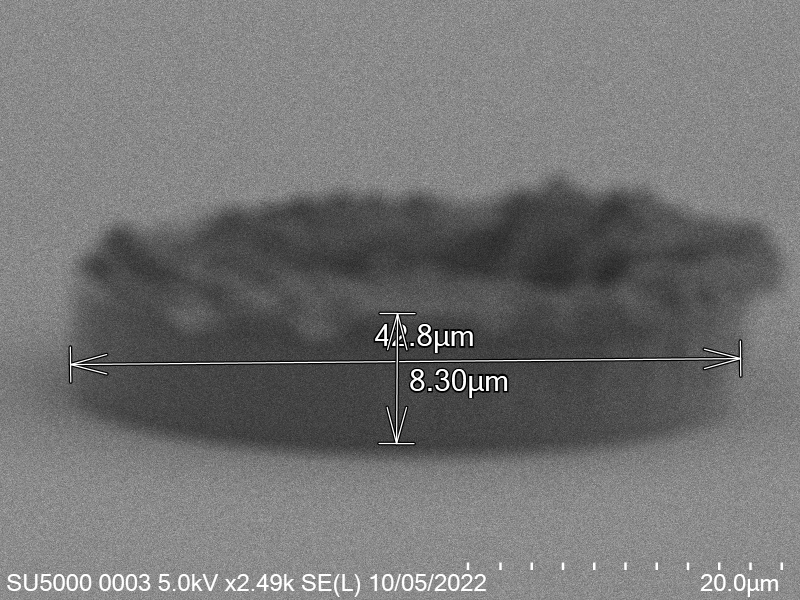
\includegraphics[width=0.65\textwidth]{Main/Ch2/indium_bump_before_bond.png}
    \caption{SEM image of indium bump at an angle of $80^\circ$}
    \label{fig:semIndium}
\end{figure}

The raw data from which I determined the average indium thickness is from table \ref{table:thicknessMap}.

\begin{sidewaystable}
    \centering
    \renewcommand{\minval}{0.1}
    \renewcommand{\maxval}{3}
    \begin{tabular}{| l | c | c | c | c | c|}
    \hline
    Bond ID  &  In Bond Avg. Diameter ($\um$)  &  Indium Thickness ($\um$)  &  In Bump Width ($\um$)  &  In Bump Volume ($\um^3$)  &  Bond Estimated Thickness ($\um$)
    \\
    \hline
    \hline
    BID-005  &  58.6  & 1.3   & 42 & 1801   & \grd{0.667} \\
    BID-006  &  84    & 1.7   & 42 & 2355   & \grd{0.425} \\
    BID-008  &  200   & 14    & 42 & 19396  & \grd{0.617} \\
    BID-009  &  86    & 8.4   & 42 & 11637  & \grd{2.003} \\
    BID-010  &  105   & 8.3   & 42 & 11499  & \grd{1.328} \\
    BID-011  &  142   & 8.5   & 42 & 11776  & \grd{0.743} \\
    BID-012  &  164   & 10    & 42 & 13854  & \grd{0.655} \\
    \hline
    \hline
    \end{tabular}
    \caption{Table of estimated thickness post diebonding}
    \label{table:thicknessMap}
\end{sidewaystable}

From the table after removing outlier values, the median resulting thickness is $ ~65 \um $.

The spread values were identified from images taken from the microscope `OLYMPUS-scope3' in the packaging lab.

From the images captured by the scope \ref{fig:microscopeIndium}, we can see that the gimbal head in the lab provides sufficiently uniform bonding pressure over the bonding area. The images also show that there is spreading of the indium as the bond is formed directly as a function of the indium volume.

Knowing that the bond does spread will constrain the maximum density of \uleds \ for a given bump thickness.

\begin{wrapfigure}{R}{0.5\textwidth}
    \centering
    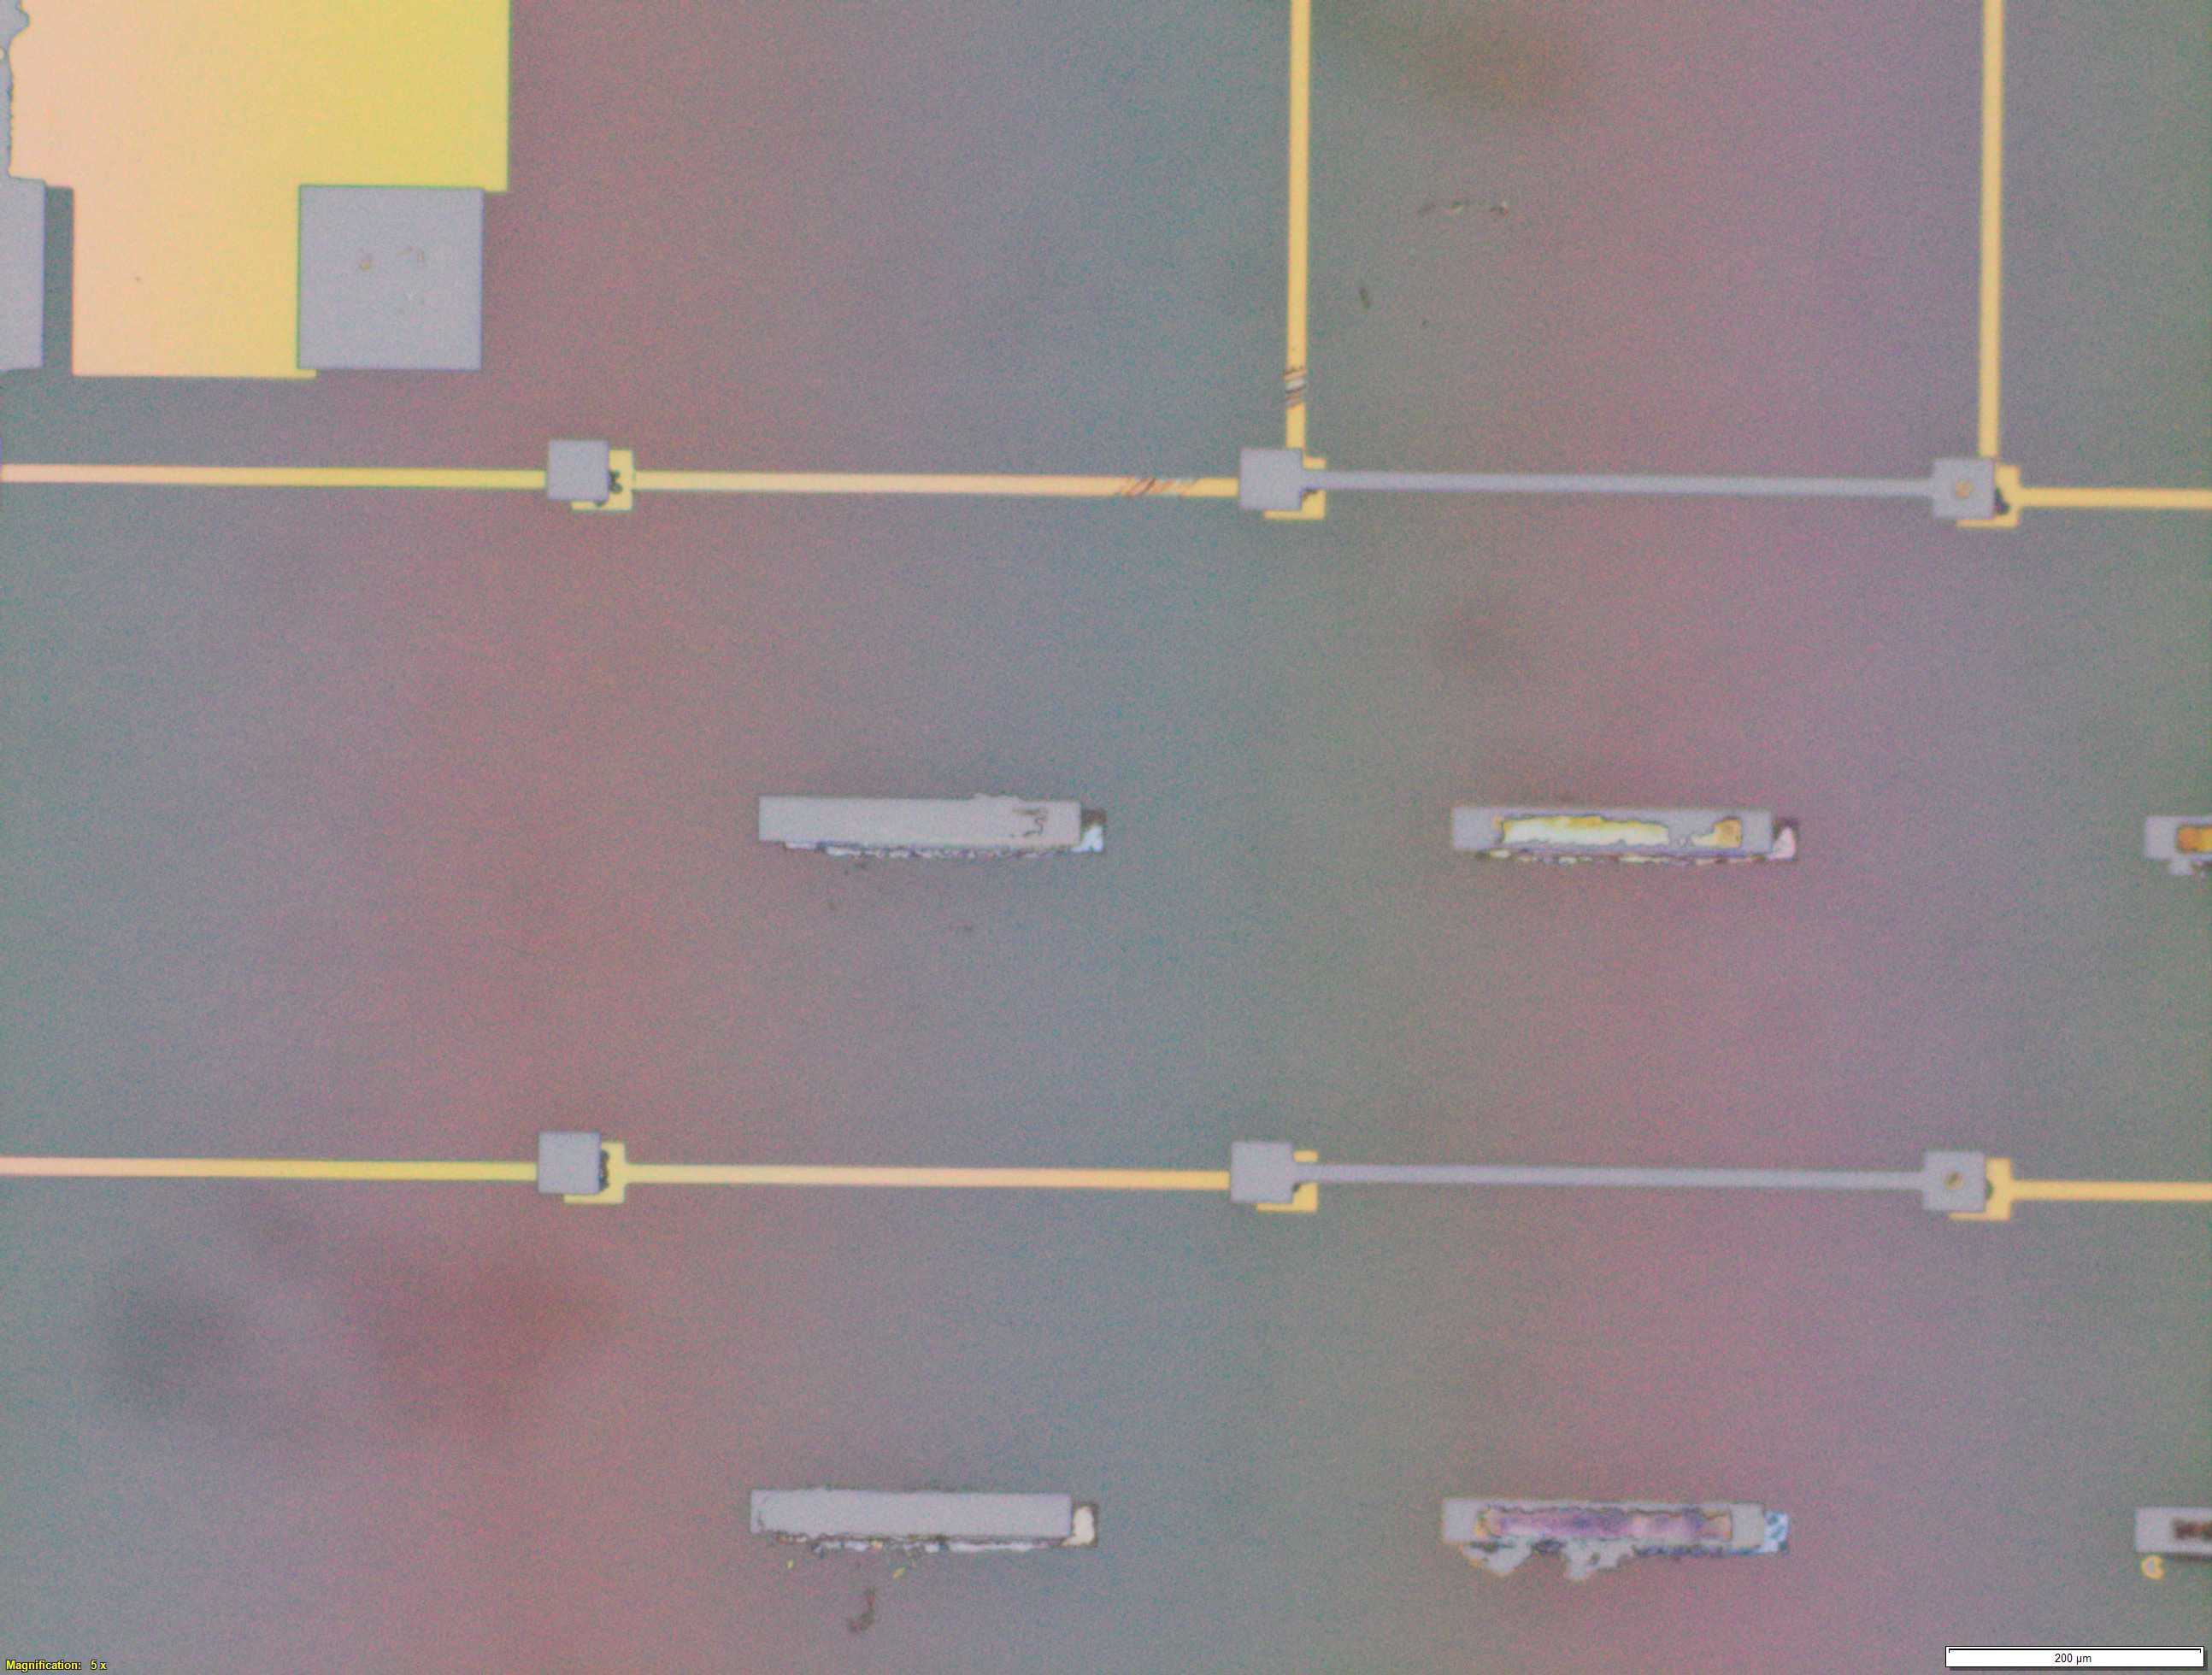
\includegraphics[width=0.22\textwidth]{Main/Ch2/TL.png}
    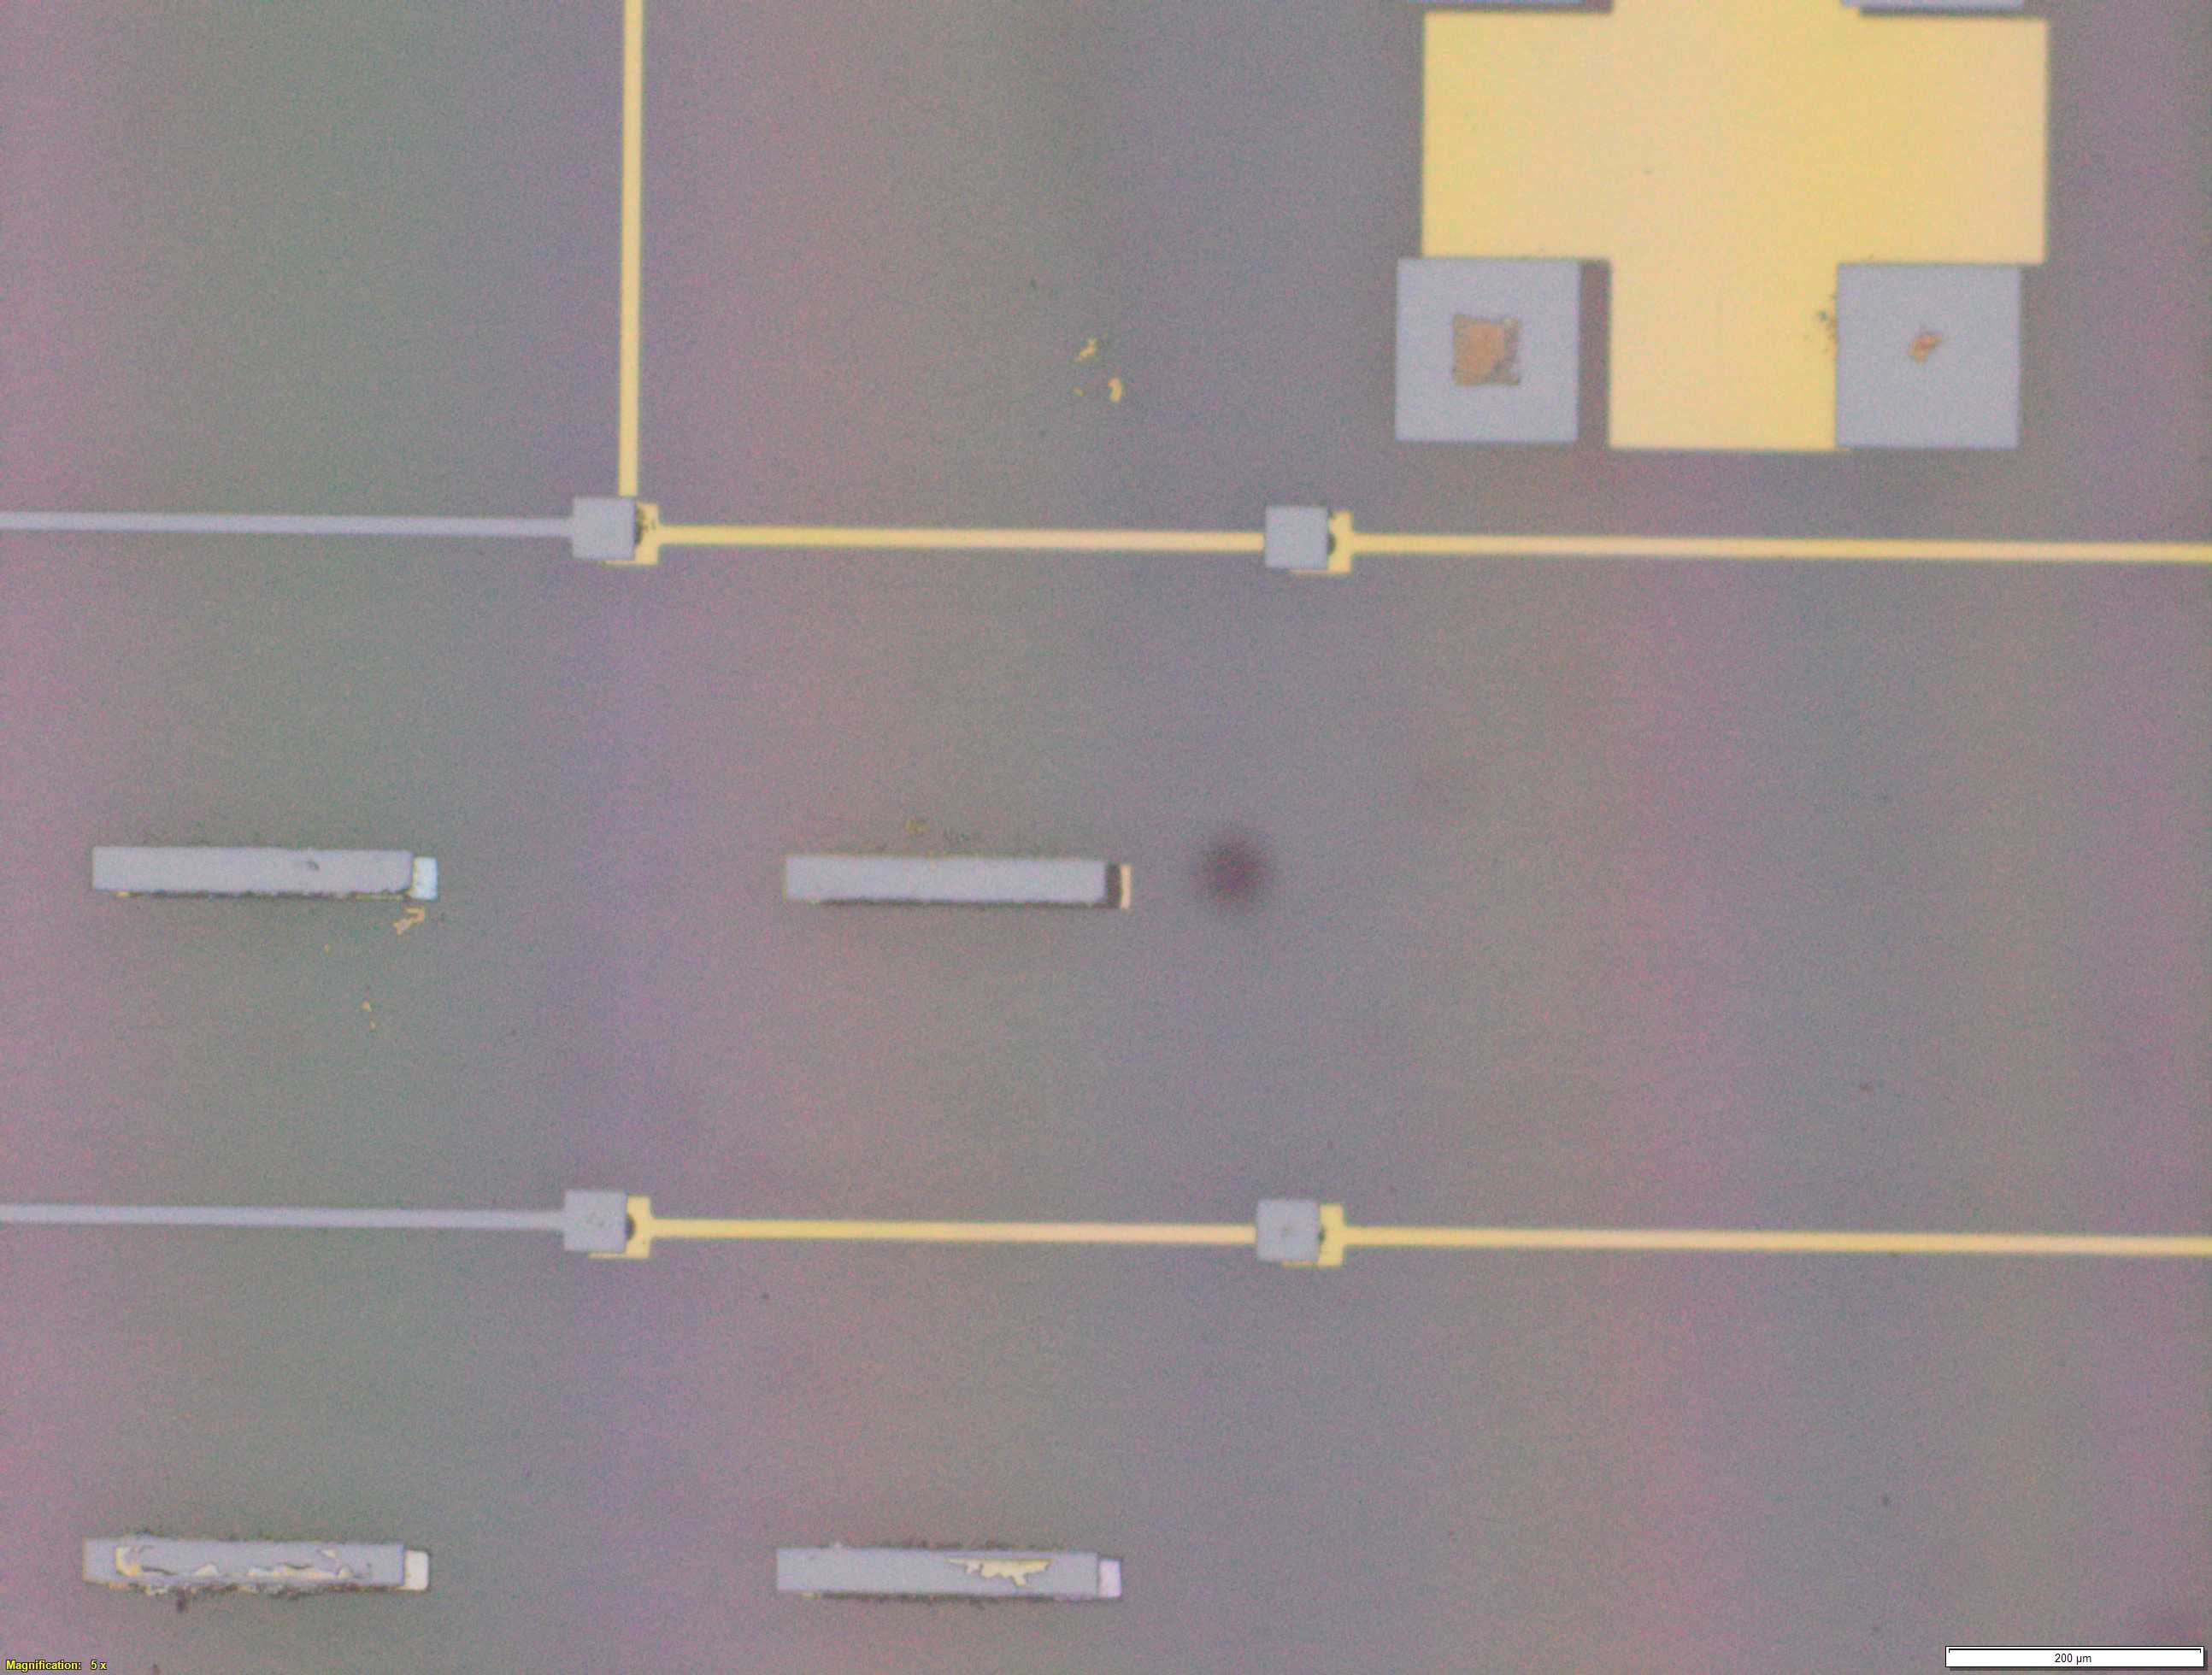
\includegraphics[width=0.22\textwidth]{Main/Ch2/TR.png} \\
    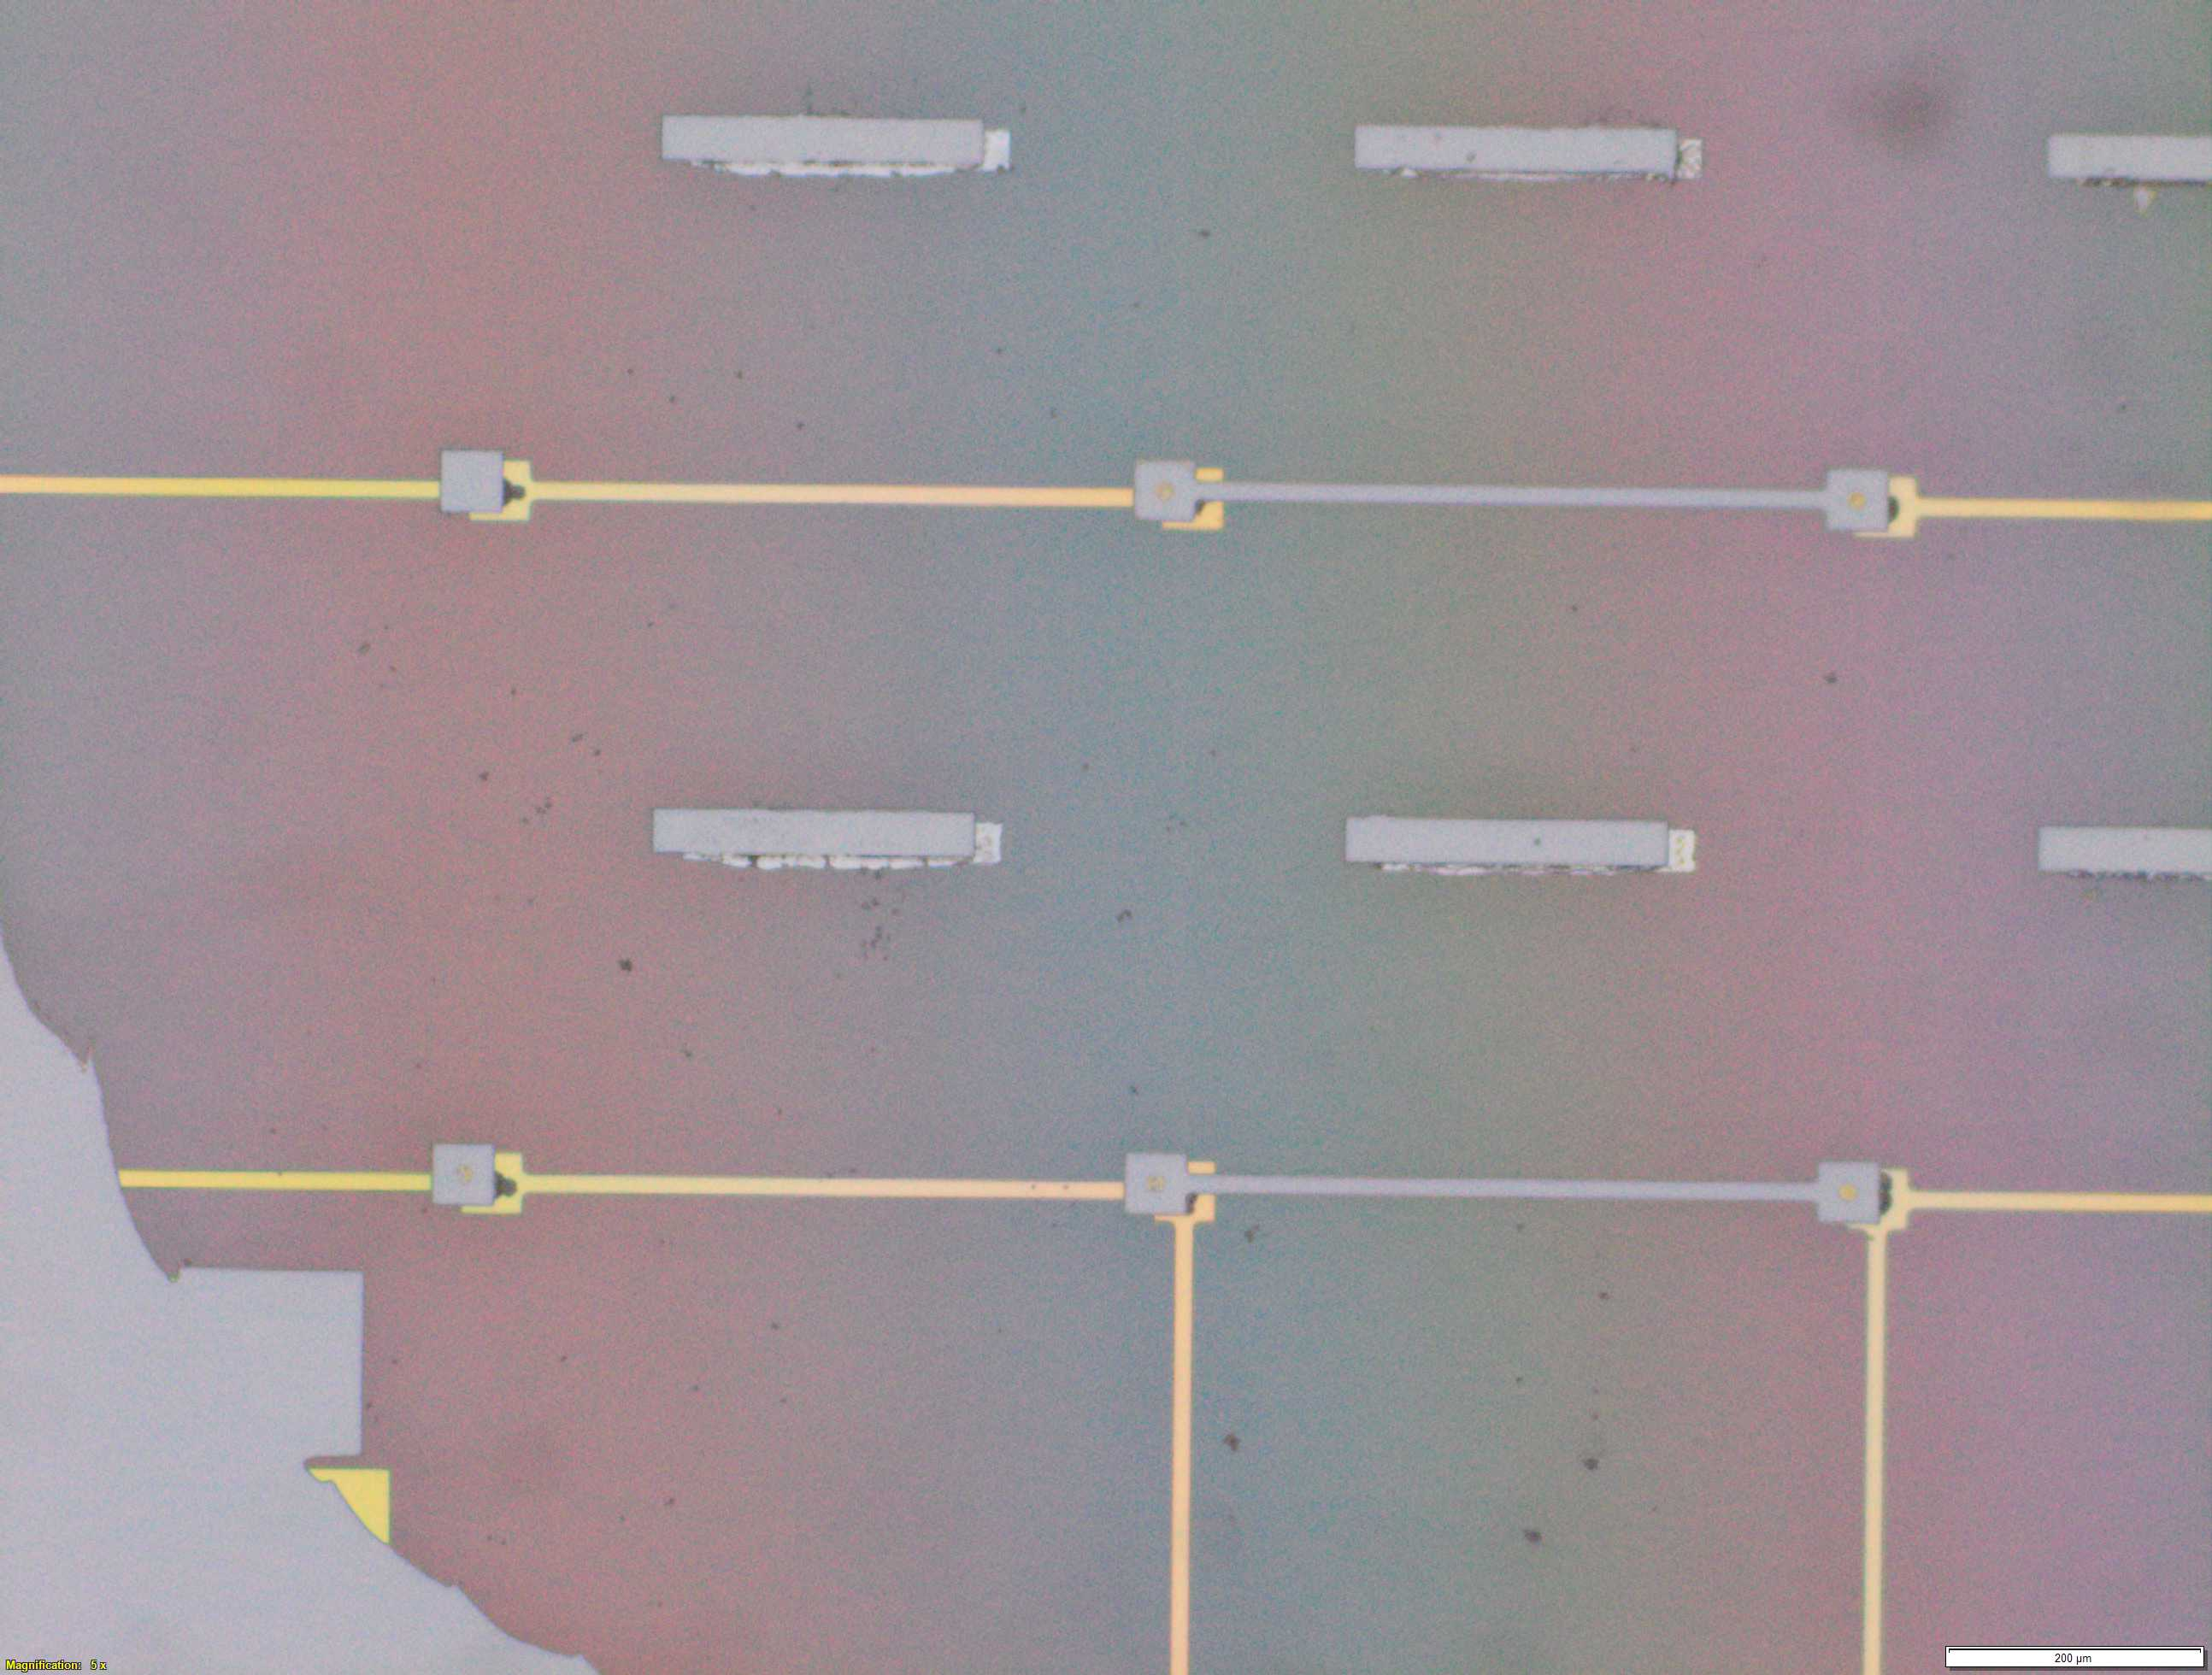
\includegraphics[width=0.22\textwidth]{Main/Ch2/BL.png}
    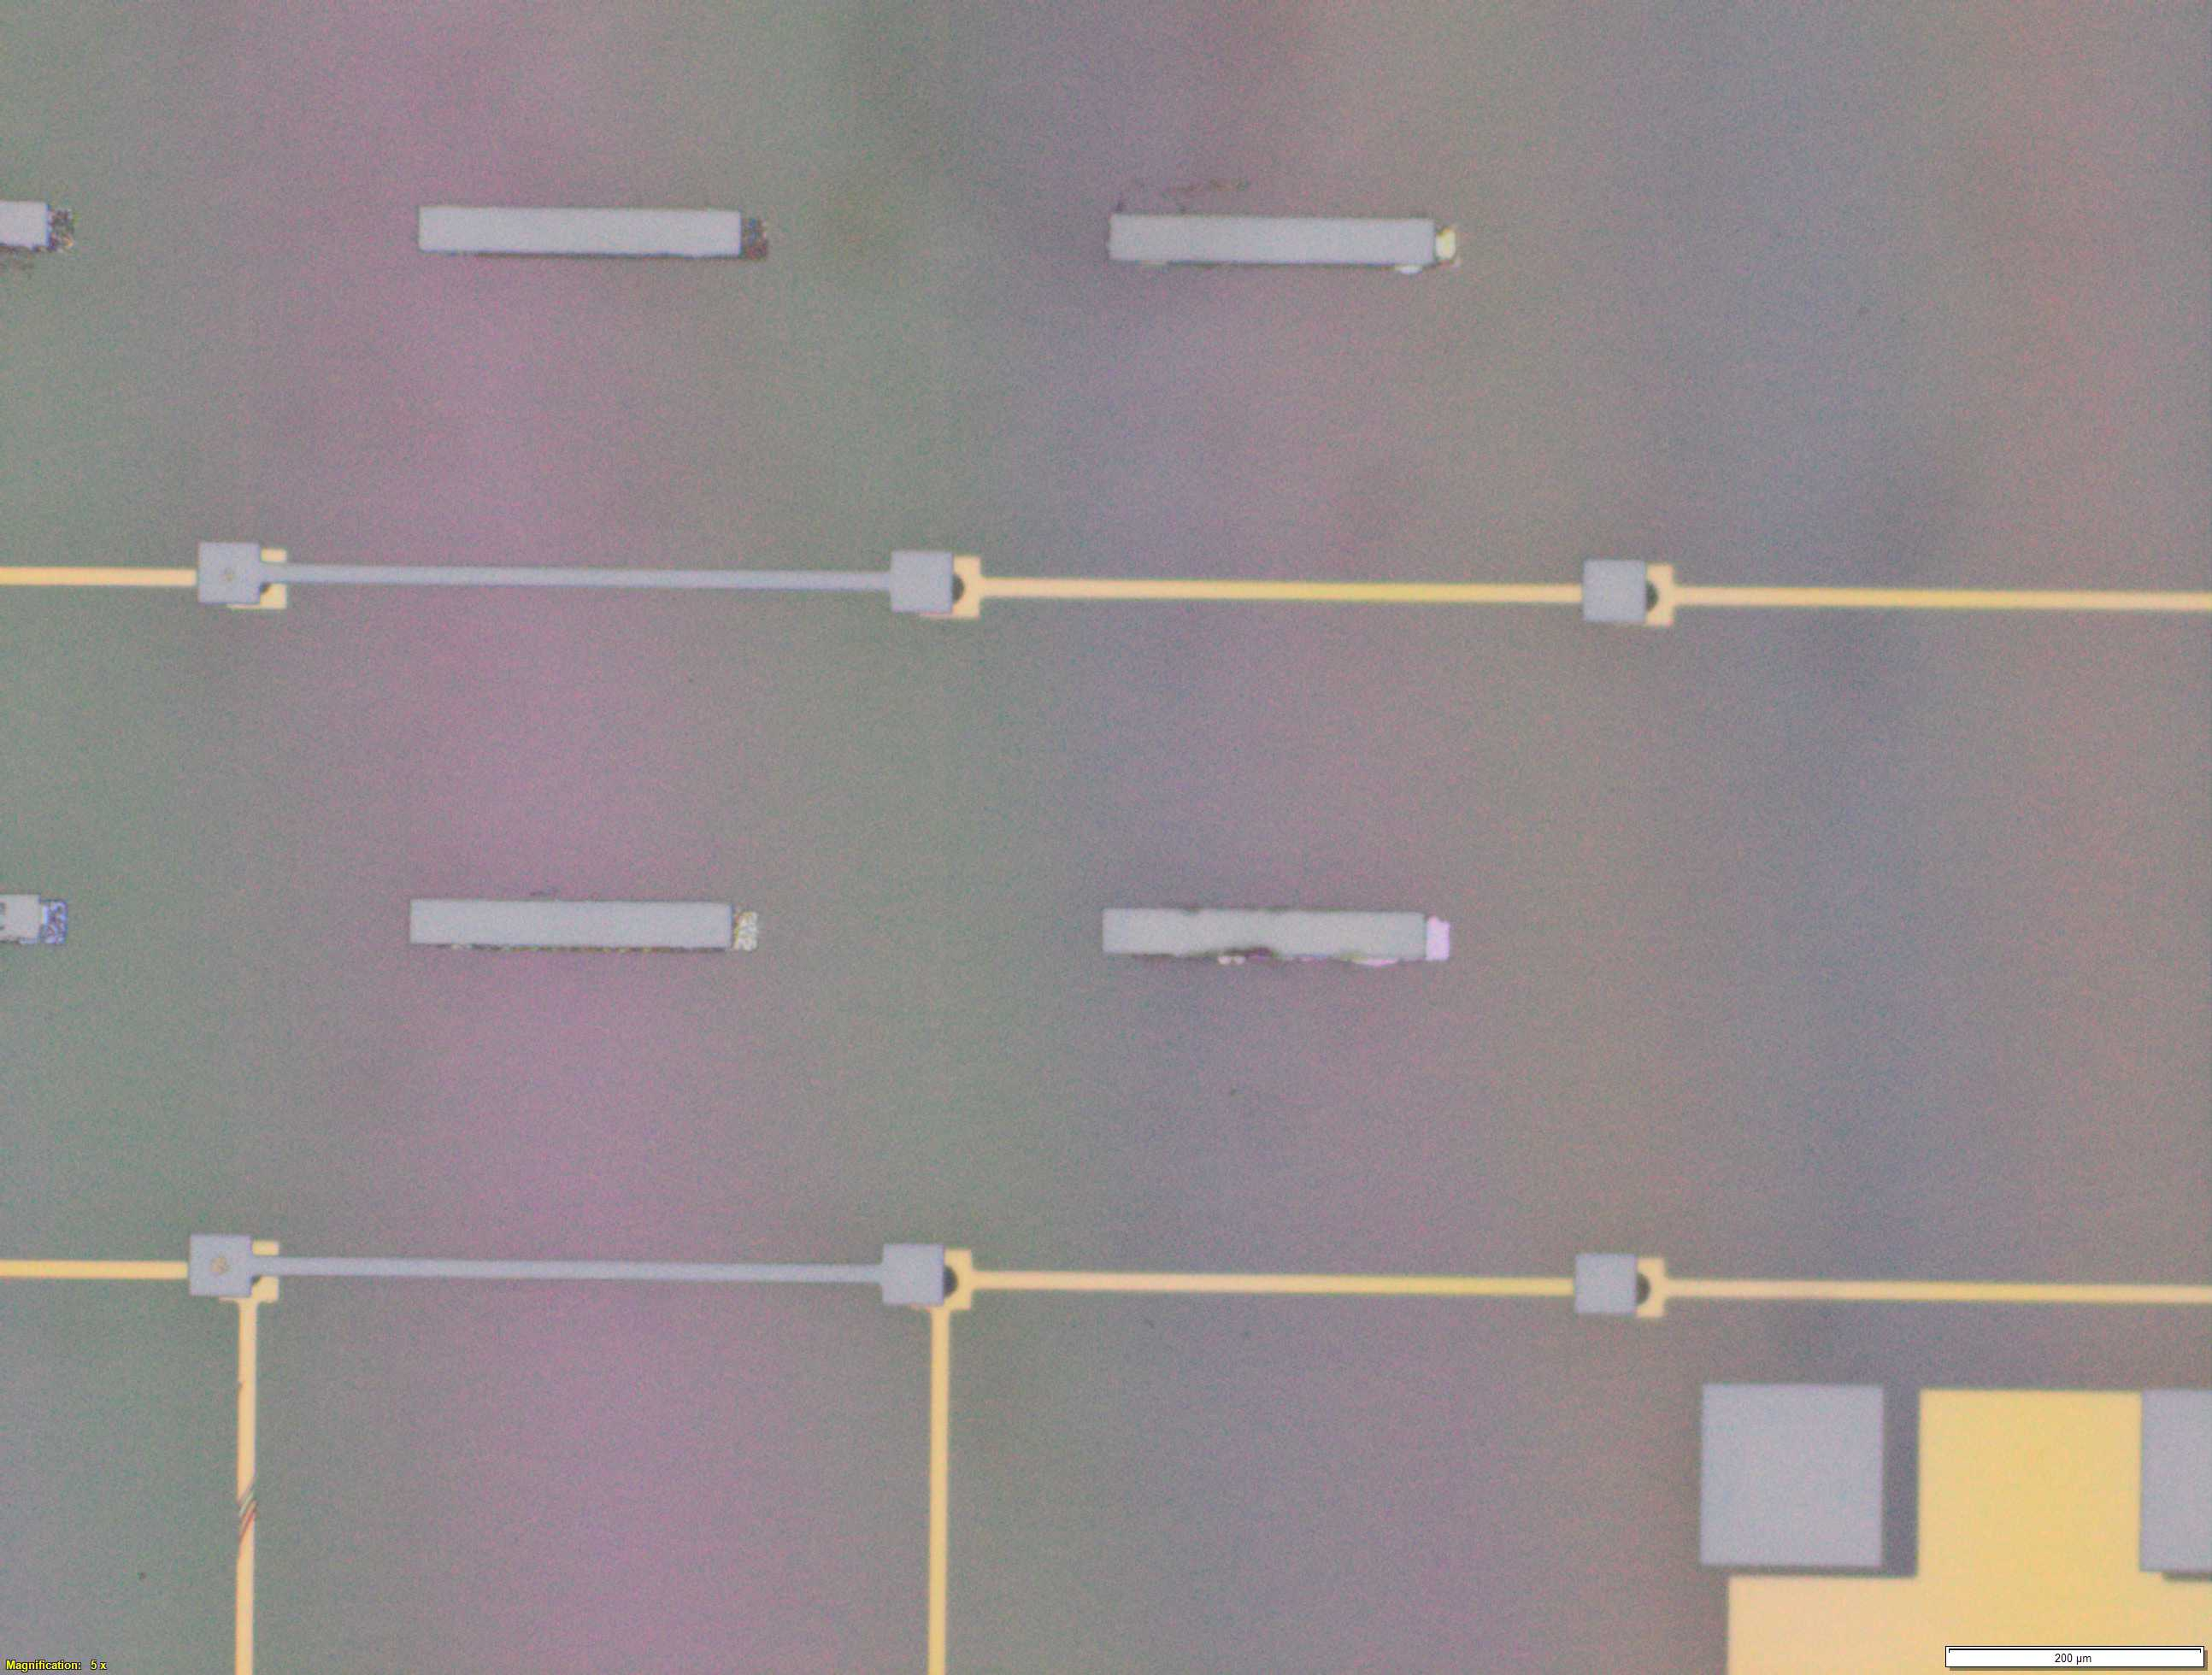
\includegraphics[width=0.22\textwidth]{Main/Ch2/BR.png}
    \caption{Microscope images of diebonded sample. The internal smaller circles seen are a diameter of $42 \um$ the larger circles are the indium spreading}
    \label{fig:microscopeIndium}
    \vspace{0.5cm}
\end{wrapfigure}

\newpage
\subsection{Validation of Uniform Bonding}
\label{sec:uniformBond}

\newpage
\subsection{Thermal Simulations}

Thermal simulations were conducted because there were some bonding failures seen in the samples. As can be seen from SEM images and Energy-dispersive X-ray spectroscopy (EDX or EDS) the indium does not always appropriately wet onto the other substrate being bonded onto this is seen in the SEM images in figure
\ref{fig:SEM_indium_2} and EDX images in figure \ref{fig:EDX_indium_2}.
There can be various reasons why indium does not wet onto a surface during diebonding. One reason could be the presence of surface contaminants such as oxides or oils, which can prevent the indium from bonding to the surface. Another reason could be an insufficient amount of heat or pressure during the diebonding process, which can cause the indium to not properly wet onto the surface. Additionally, the surface energy of the substrate can also affect the ability of indium to wet onto the surface during diebonding.

To explore further a lack of heat, thermal simulations were conducted to identify if a process change in the diebonding preprocess was required. Thermal simulations were done in MATLAB with the following code in
\hyperref[sec:ThermalSimulationCode]{Appendix B}.


\begin{wrapfigure}{L}{0.45\textwidth}
    \centering
    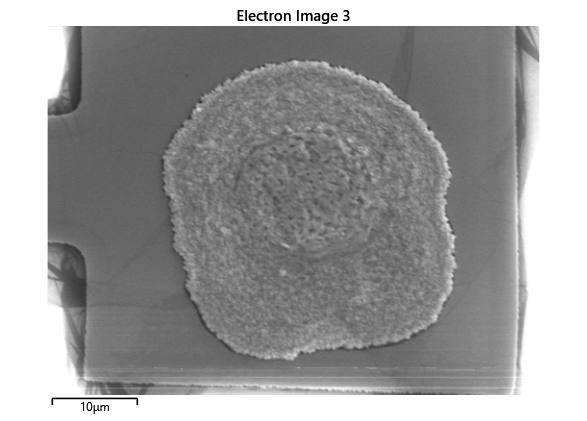
\includegraphics[width=0.1\textwidth]{Main/Ch2/extracted/SEM/In-EP-EDx_TBP-01-A1-s1_media_image.png}
    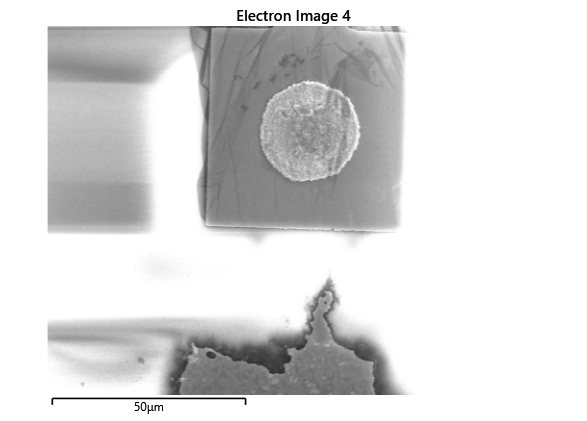
\includegraphics[width=0.1\textwidth]{Main/Ch2/extracted/SEM/In-EP-EDx_TBP-01-A1-s2_media_image.png}
    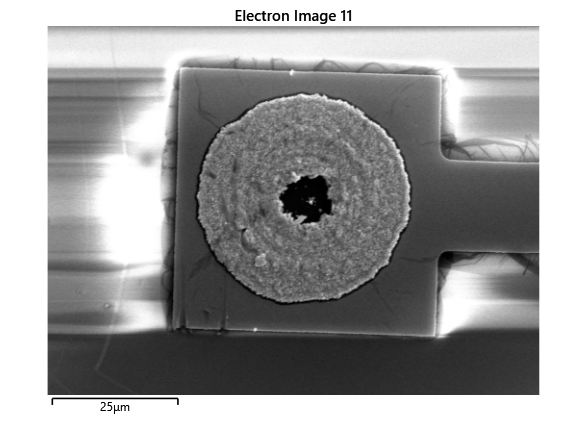
\includegraphics[width=0.1\textwidth]{Main/Ch2/extracted/SEM/In-EP-EDx_TBP-01-A2-s1_media_image.png}
    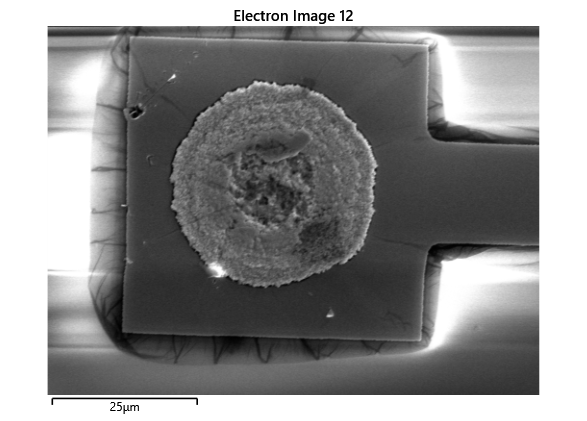
\includegraphics[width=0.1\textwidth]{Main/Ch2/extracted/SEM/In-EP-EDx_TBP-01-A2-s2_media_image.png}
    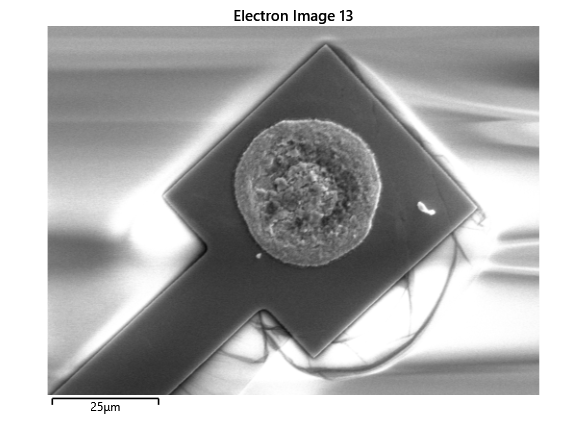
\includegraphics[width=0.1\textwidth]{Main/Ch2/extracted/SEM/In-EP-EDx_TBP-01-B2-s1_media_image.png}
    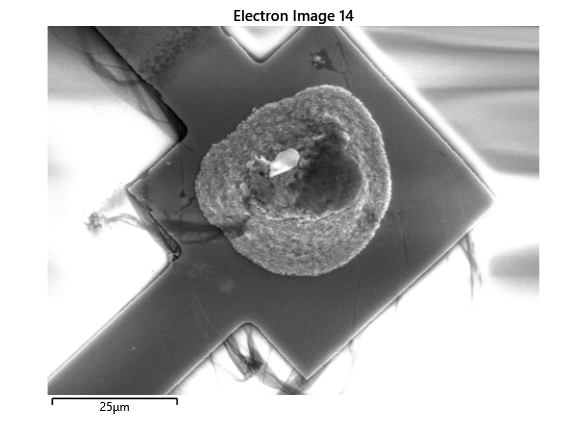
\includegraphics[width=0.1\textwidth]{Main/Ch2/extracted/SEM/In-EP-EDx_TBP-01-B2-s2_media_image.png}
    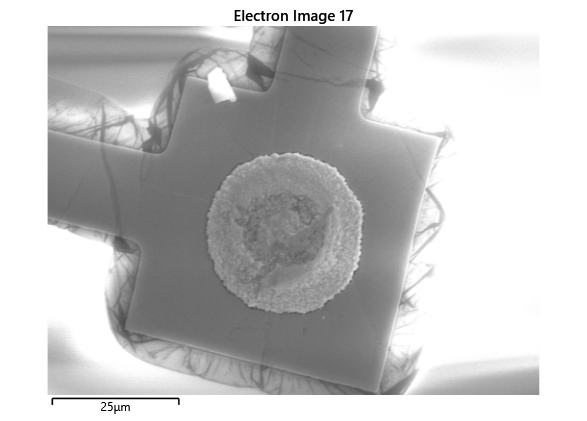
\includegraphics[width=0.1\textwidth]{Main/Ch2/extracted/SEM/In-EP-EDx_TBP-02-A1-s1_media_image.png}
    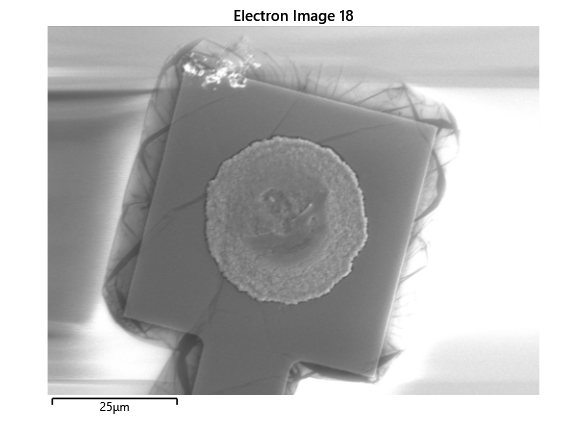
\includegraphics[width=0.1\textwidth]{Main/Ch2/extracted/SEM/In-EP-EDx_TBP-02-A1-s2_media_image.png}
    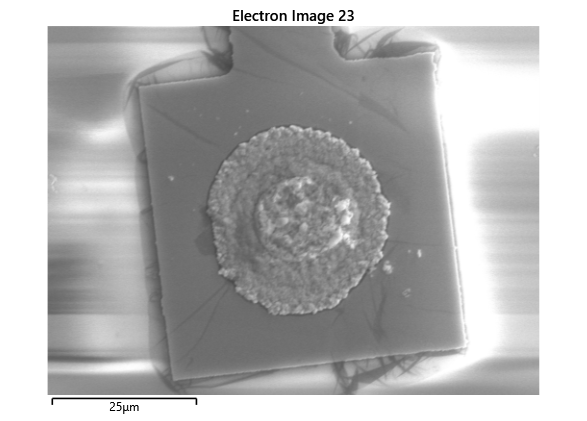
\includegraphics[width=0.1\textwidth]{Main/Ch2/extracted/SEM/In-EP-EDx_TBP-02-A2-s1_media_image.png}
    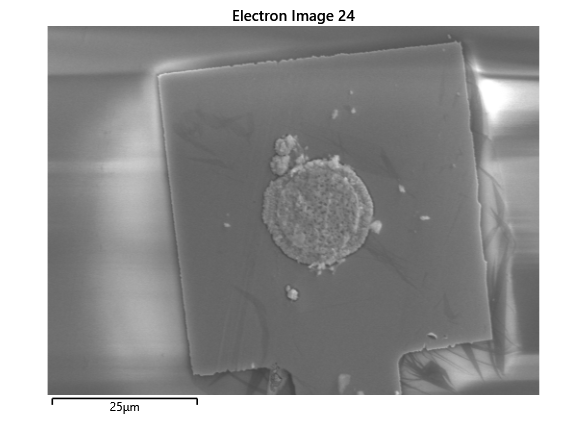
\includegraphics[width=0.1\textwidth]{Main/Ch2/extracted/SEM/In-EP-EDx_TBP-02-A2-s2_media_image.png}
    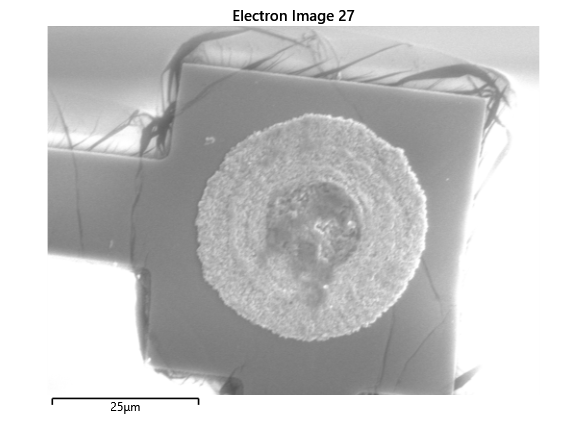
\includegraphics[width=0.1\textwidth]{Main/Ch2/extracted/SEM/In-EP-EDx_TBP-02-B2-s1_media_image.png}
    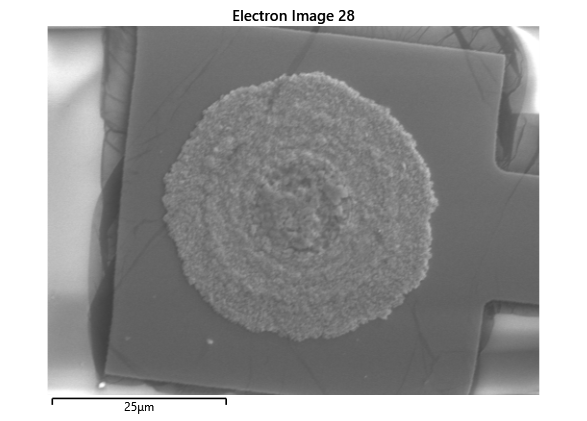
\includegraphics[width=0.1\textwidth]{Main/Ch2/extracted/SEM/In-EP-EDx_TBP-02-B2-s2_media_image.png}
    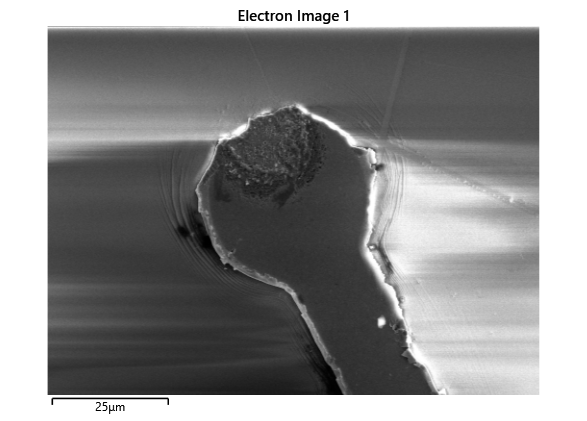
\includegraphics[width=0.1\textwidth]{Main/Ch2/extracted/SEM/In-EP-EDx_TLED-01-A1-s1_media_image.png}
    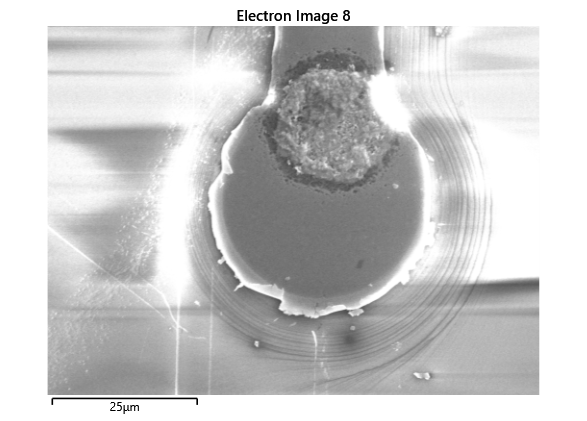
\includegraphics[width=0.1\textwidth]{Main/Ch2/extracted/SEM/In-EP-EDx_TLED-01-A1-s2_media_image.png}
    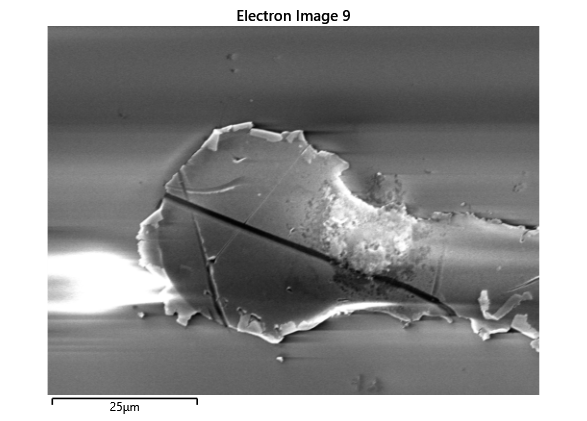
\includegraphics[width=0.1\textwidth]{Main/Ch2/extracted/SEM/In-EP-EDx_TLED-01-A2-s1_media_image.png}
    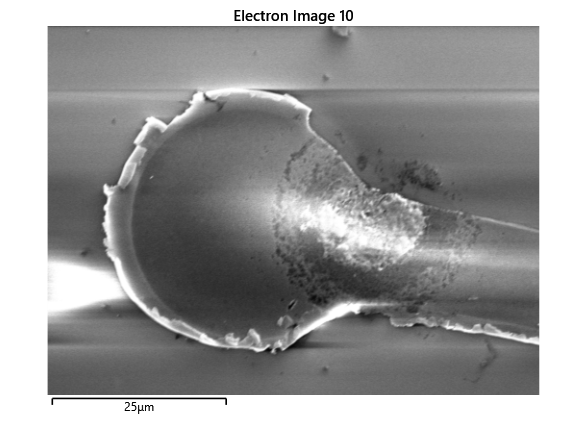
\includegraphics[width=0.1\textwidth]{Main/Ch2/extracted/SEM/In-EP-EDx_TLED-01-A2-s2_media_image.png}
    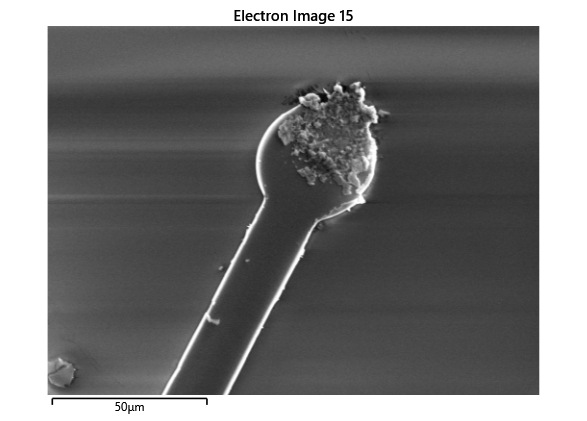
\includegraphics[width=0.1\textwidth]{Main/Ch2/extracted/SEM/In-EP-EDx_TLED-01-B2-s1_media_image.png}
    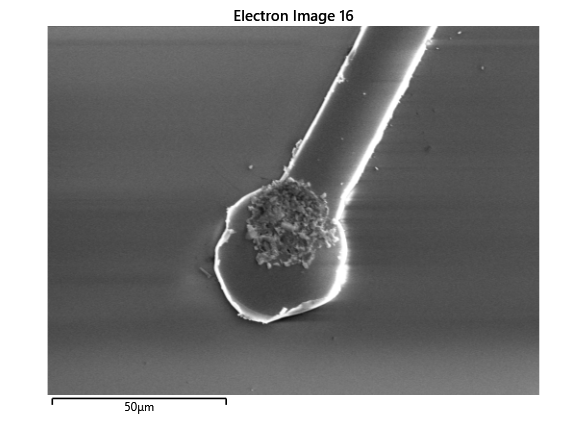
\includegraphics[width=0.1\textwidth]{Main/Ch2/extracted/SEM/In-EP-EDx_TLED-01-B2-s2_media_image.png}
    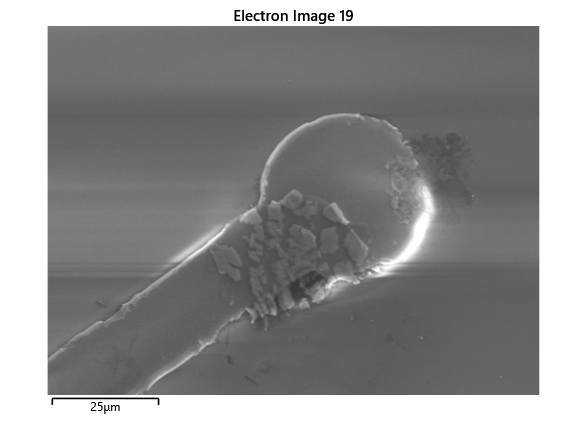
\includegraphics[width=0.1\textwidth]{Main/Ch2/extracted/SEM/In-EP-EDx_TLED-02-A1-s1_media_image.png}
    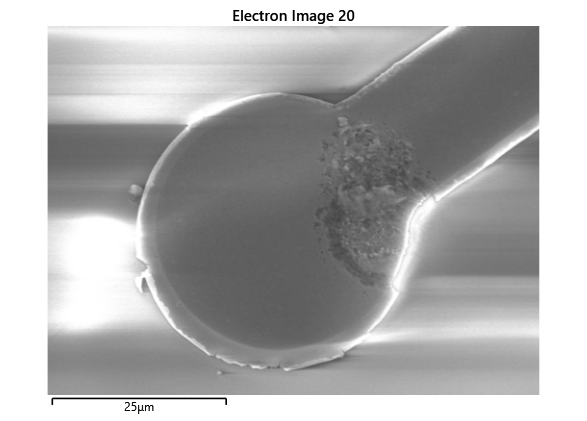
\includegraphics[width=0.1\textwidth]{Main/Ch2/extracted/SEM/In-EP-EDx_TLED-02-A1-s2_media_image.png}
    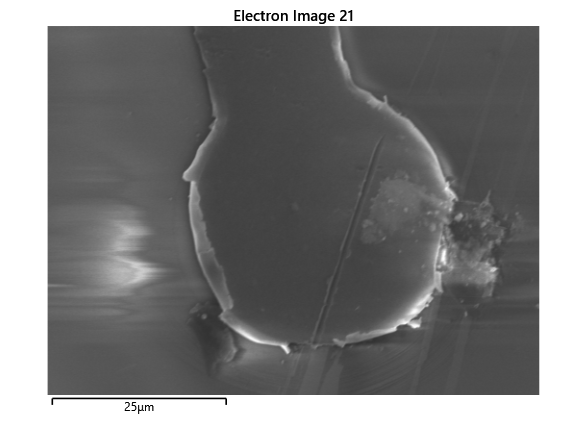
\includegraphics[width=0.1\textwidth]{Main/Ch2/extracted/SEM/In-EP-EDx_TLED-02-A2-s1_media_image.png}
    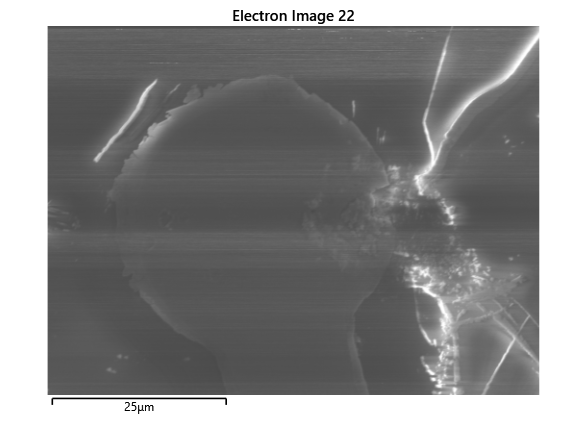
\includegraphics[width=0.1\textwidth]{Main/Ch2/extracted/SEM/In-EP-EDx_TLED-02-A2-s2_media_image.png}
    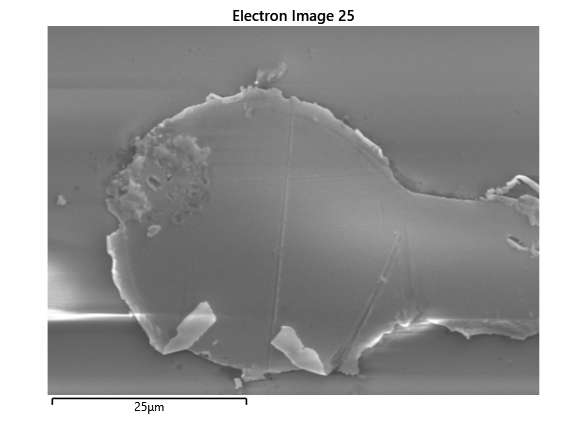
\includegraphics[width=0.1\textwidth]{Main/Ch2/extracted/SEM/In-EP-EDx_TLED-02-B2-s1_media_image.png}
    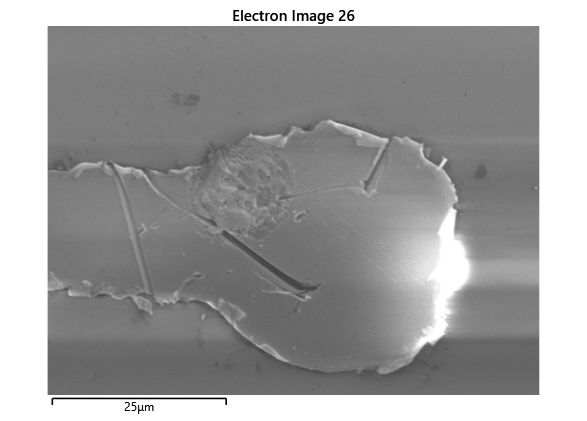
\includegraphics[width=0.1\textwidth]{Main/Ch2/extracted/SEM/In-EP-EDx_TLED-02-B2-s2_media_image.png}
    \caption{SEM Images of bonds}
    \label{fig:SEM_indium_2}
    \vspace{0.5cm}
\end{wrapfigure}


\begin{wrapfigure}{R}{0.45\textwidth}
    \centering
    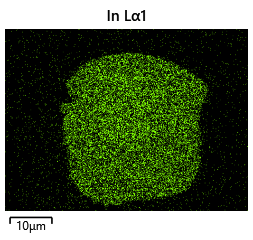
\includegraphics[width=0.1\textwidth]{Main/Ch2/extracted/Indium/In-EP-EDx_TBP-01-A1-s1_media_image7.png}
    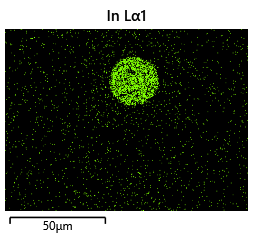
\includegraphics[width=0.1\textwidth]{Main/Ch2/extracted/Indium/In-EP-EDx_TBP-01-A1-s2_media_image7.png}
    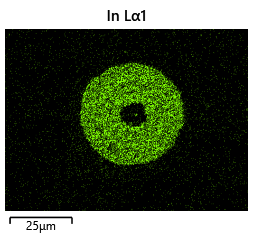
\includegraphics[width=0.1\textwidth]{Main/Ch2/extracted/Indium/In-EP-EDx_TBP-01-A2-s1_media_image7.png}
    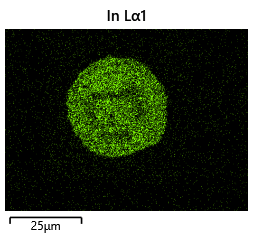
\includegraphics[width=0.1\textwidth]{Main/Ch2/extracted/Indium/In-EP-EDx_TBP-01-A2-s2_media_image7.png}
    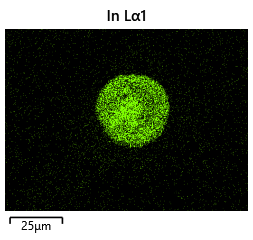
\includegraphics[width=0.1\textwidth]{Main/Ch2/extracted/Indium/In-EP-EDx_TBP-01-B2-s1_media_image7.png}
    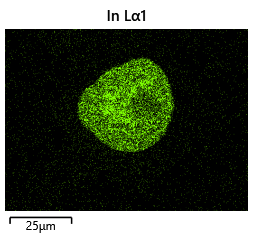
\includegraphics[width=0.1\textwidth]{Main/Ch2/extracted/Indium/In-EP-EDx_TBP-01-B2-s2_media_image7.png}
    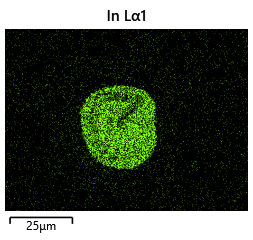
\includegraphics[width=0.1\textwidth]{Main/Ch2/extracted/Indium/In-EP-EDx_TBP-02-A1-s1_media_image7.png}
    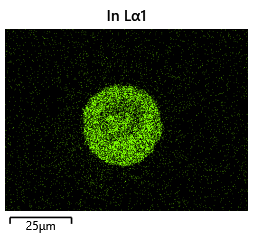
\includegraphics[width=0.1\textwidth]{Main/Ch2/extracted/Indium/In-EP-EDx_TBP-02-A1-s2_media_image7.png}
    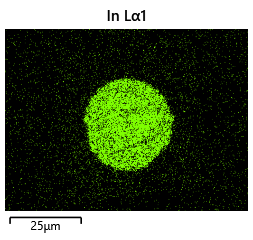
\includegraphics[width=0.1\textwidth]{Main/Ch2/extracted/Indium/In-EP-EDx_TBP-02-A2-s1_media_image7.png}
    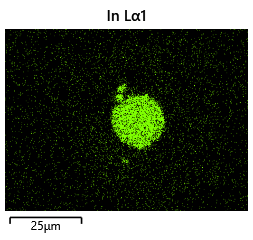
\includegraphics[width=0.1\textwidth]{Main/Ch2/extracted/Indium/In-EP-EDx_TBP-02-A2-s2_media_image7.png}
    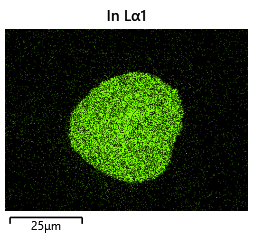
\includegraphics[width=0.1\textwidth]{Main/Ch2/extracted/Indium/In-EP-EDx_TBP-02-B2-s1_media_image7.png}
    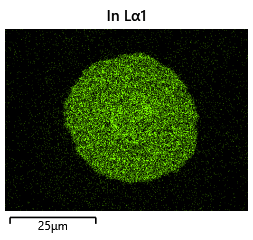
\includegraphics[width=0.1\textwidth]{Main/Ch2/extracted/Indium/In-EP-EDx_TBP-02-B2-s2_media_image7.png}
    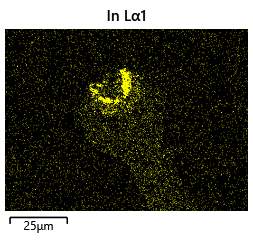
\includegraphics[width=0.1\textwidth]{Main/Ch2/extracted/Indium/In-EP-EDx_TLED-01-A1-s1_media_image7.png}
    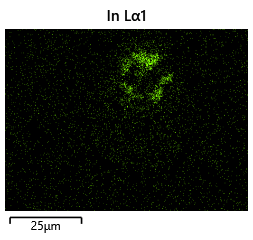
\includegraphics[width=0.1\textwidth]{Main/Ch2/extracted/Indium/In-EP-EDx_TLED-01-A1-s2_media_image7.png}
    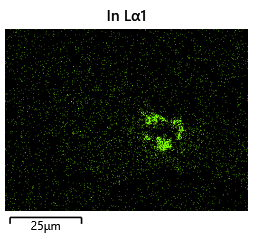
\includegraphics[width=0.1\textwidth]{Main/Ch2/extracted/Indium/In-EP-EDx_TLED-01-A2-s1_media_image7.png}
    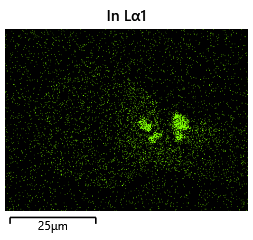
\includegraphics[width=0.1\textwidth]{Main/Ch2/extracted/Indium/In-EP-EDx_TLED-01-A2-s2_media_image7.png}
    \includegraphics[width=0.1\textwidth]{Main/Ch2/extracted/Indium/In-EP-EDx_TLED-01-B2-s1_media_image7.png}
    \includegraphics[width=0.1\textwidth]{Main/Ch2/extracted/Indium/In-EP-EDx_TLED-01-B2-s2_media_image7.png}
    \includegraphics[width=0.1\textwidth]{Main/Ch2/extracted/Indium/In-EP-EDx_TLED-02-A1-s1_media_image7.png}
    \includegraphics[width=0.1\textwidth]{Main/Ch2/extracted/Indium/In-EP-EDx_TLED-02-A1-s2_media_image7.png}
    \includegraphics[width=0.1\textwidth]{Main/Ch2/extracted/Indium/In-EP-EDx_TLED-02-A2-s1_media_image7.png}
    \includegraphics[width=0.1\textwidth]{Main/Ch2/extracted/Indium/In-EP-EDx_TLED-02-A2-s2_media_image7.png}
    \includegraphics[width=0.1\textwidth]{Main/Ch2/extracted/Indium/In-EP-EDx_TLED-02-B2-s1_media_image7.png}
    \includegraphics[width=0.1\textwidth]{Main/Ch2/extracted/Indium/In-EP-EDx_TLED-02-B2-s2_media_image7.png}
    \caption{EDX Images of bonds}
    \label{fig:EDX_indium_2}
\end{wrapfigure}


The results from the thermal simulations as seen in figure \ref{fig:thermal_simulations} in MATLAB were that there was more than sufficient time and heat to melt and wet the indium onto the opposing surface. As a result the lack of wetting was likely a result of one of the other issues (contaminants from the flip-chip process or some failure in the surface energies).
Both of the other issues are quite possible as during the process the substrate that is bonding onto the substrate with indium on the surface is face down on the `diebonder' which is an unclean surface that also does not have the appropriate surface energies and could dissipate the surface energy generated during the plasma cleaning process.
% TODO Verify statement about suface energy

It can be seen from the thermal simulations that the time taken for the indium to reach temperature is well within $0.3 \unit{\second}$ whereas the bonding recipe calls for the sample to sit at $250 \dC$ for $5 \unit{\minute}$. This is well within 2 orders of magnitude of time for the sample to reach temperature, as such it would be safe to assume that heat/temperature or lack thereof is not the causal source of failure.


\begin{wrapfigure}{L}{0.5\textwidth}
    \centering
    \includegraphics[width=0.21\textwidth]{Main/Ch2/heat/001.png}
    \includegraphics[width=0.21\textwidth]{Main/Ch2/heat/002.png}
    \includegraphics[width=0.21\textwidth]{Main/Ch2/heat/008.png}
    \includegraphics[width=0.21\textwidth]{Main/Ch2/heat/020.png}
    \caption{Thermal simulation results. Temperature scale is ranged from $25 \dC$ to $250 \dC$}
    \label{fig:thermal_simulations}
\end{wrapfigure}


\subsection{Conformation to Theory}
In this section we wanted to ensure that there was uniform bonding across the area of the sample, this would arise from the bonding head providing relatively uniform bonding force over the sample area. From the microscope images in \ref{fig:microscopeIndium} we can see that the spread of the indium bumps is uniform over the area of the sample, this would be representative of the gimbal head providing relatively uniform pressure over the face of the sample.

Conformed to theory when the bonding would spread according to the calculated volume.

\subsection{Development of a Repeatable Process}
% Adding anchors
\newpage
\chapter{Phase 2 - Electrical Connection}
\label{sec:Ch3_elec}

\section{Process}

\section{Characterization of Electrical Connection}
Conducting the daisychain test

\section{Connection Issues}
did not connect at first,

% Keeping process temperature low
adjusted process to not do hmds

\section{Conformation to Theory}
\section{Development of a Repeatable Process}


\subsection{Improving cleanliness of process}

I acquired a 4-inch wafer to place the LED on while it was being picked up for diebonding. The wafer is also surface activated and placed in the plasma cleaner with the rest of the samples to ensure it is also relatively clean. The wafer when not being used is placed in the wafer carrier tray. Furthermore, the bonding head is regularly cleaned with IPA before being used.
% Plasma clean
% Clean Wafer
\newpage
\chapter{Phase 3 - Bonding to LEDs}
\label{sec:BondingToLEDS}
\section{Bonding Issues}
\section{Lighting Issues}
\section{Conformation to Theory}
\section{Development of a Repeatable Process}

\newpage
\section{Addendum - Driving Displays}
\subsection{Passive Matrix Displays}
\subsection{Active Matrix Displays}
\subsection{Designs for In-House drivers}

\pagebreak
\printbibliography
\pagebreak
\section{Appendix}
\subsection{Appendix A - Standard Operating Procedure Electroplating E3}
\label{sec:SOP}

\begin{center} % center the minipage
    \begin{framed} % add a border to the minipage
        \begin{minipage}{0.8\textwidth} % set the width of the minipage
            \raggedright % align the text to the left
            \textbf{Note}: Electroplating procedure used in the E3-3139 Lab

            \vspace{0.1cm} % add some vertical space between the title and the body of the minipage

            \mpsection{Purpose}
            Depositing Indium from an electroplating solution onto samples for die-bonding. The solution used is from Indium Corporation of America and uses their Indium Sulfamate Plating Kit to perform the Indium electroplating.

            \mpsection{Equipment}
            \begin{center}

            \begin{tabular}{|l|c|}
                \hline
                \textbf{Name}  &   \textbf{Quantity} \\
                \hline
                Fume Hood                           &	1 \\
                N2 Gun                              &	1 \\
                DI Water Bottle                     &	1 \\
                2L Beakers                          &	2 \\
                400mL Beaker                        &	1 \\
                200mL Beaker                        &	1 \\
                1L HDPE Bottle                      &	1 \\
                500mL HDPE Bottle                   &	1 \\
                Hotplate with Magnetic Stirring     &	1 \\
                Magnetic Stir Bar                   &   1 \\
                Funnel                              &	1 \\
                Insulated Copper Wire               &	2 \\
                Banana Plug Wires                   &	2 \\
                Copper Alligator Clips              &	2 \\
                Tweezers kit                        &	1 \\
                Custom Sample Holder                &	1 \\
                \hline
            \end{tabular}

            \vspace{0.5cm}

            \begin{tabular}{|l|c|}
                \hline
                \textbf{Name} & \textbf{Quantity} \\
                \hline
                Indium Sulfamate Plating Bath        & 1L \\
                Indium Anode (30cm x 2.5cm x 1.5mm)  & 1 \\
                Sulfamic Acid                        & 150mL \\
                15-20\% HCl                          & 150mL \\
                DI Water                             & 10L \\
                pH Paper Set or pH Meter             & 1 \\
                Clean Room Wipes Pack                & 1 \\
                \hline
            \end{tabular}

            \end{center}

        \end{minipage}
    \end{framed}
\end{center}


\begin{center} % center the minipage
    \begin{framed} % add a border to the minipage
        \begin{minipage}{0.8\textwidth} % set the width of the minipage
            \raggedright % align the text to the left
            \setcounter{mpsection}{2}

            \mpsection{Chemical Hazards}

            No new chemicals are being introduced into the lab, and the SDS of the chemicals relevant to the experiment are attached with the following SOP.

            \begin{itemize}
                \item Sulfamic Acid
                \item Indium Sulfamate Plating Bath
            \end{itemize}

            \mpsection{Safety Procedure}
            \begin{itemize}
                \item Lab apron, rubber gloves, safety goggles, face-shield, and closed-toed shoes must be worn before interacting with any chemicals
                \item To avoid spills ready all beakers and bottles under the fume-hood over clean room wipes before opening
                \item Use care when opening and pouring chemicals to avoid spills during the preparation and process of the experiment
                \item Do not touch your face or exposed skin during the process of the experiment
                \item Always wash hands after handling any chemicals or materials
                \item Avoid inhaling the mist or vapor of the chemicals, and avoid exposure to eyes and skin
                \item Perform the entire experiment under a fume hood
            \end{itemize}
        \end{minipage}
    \end{framed}
\end{center}


\begin{center} % center the minipage
    \begin{framed} % add a border to the minipage
        \begin{minipage}{0.8\textwidth} % set the width of the minipage
            \raggedright % align the text to the left
            \setcounter{mpsection}{4}
            \mpsection{Process Flow}
            \begin{enumerate}
                \item Prepare the fume hood surface:
                \begin{enumerate}
                    \item Place clean room wipes on the surface of the fume hood.
                    \item Ensure your name and contact information are visible at the work location in case people need to contact you.
                    \item Chemicals in the beakers should be identified and all beakers should be labeled with what chemicals will be in them.
                \end{enumerate}
                \item Place the digital hotplate with stirring functionality inside the fume hood.
                \begin{enumerate}
                    \item Do not place a wipe on the hotplate surface. This interferes with the transmission of heat to the beaker and its contents. It may also present a fire hazard. This is regardless of weather the heating element will be used.
                    \item Do NOT turn on the heating element over the course of this experiment.
                \end{enumerate}
                \item Set all four beakers (2x 2L, 1x 400mL, 1x 200mL) under the fume hood, and set one 2L beaker on the hotplate. Place the stir bar inside the beaker on the hotplate.
                \item Build the Custom Sample Holder and place in the beaker on the hotplate at the appropriate distance for the electroplating process (~5cm).
                \item Place the indium anode into the beaker on the hotplate, ensure that there is an appropriate distance from the sample and ensure that the electrode is connected to an alligator clip. Be sure to use fresh gloves when handling the indium electrode to avoid contamination.
                \begin{enumerate}
                    \item Anode/cathode distance may alter grain size and uniformity of electroplating.
                    \item It is essential that the sample is perpendicular to the normal of the anode (indium)
                \end{enumerate}

                \item Ensure that all PPE is worn appropriately, and no skin is exposed.
                \item Acquire the indium sulfamate solution, sulfamic acid, and diluted HCl solutions from the Acids cabinet and transport it to the fume hood.
                \begin{enumerate}
                    \item Pour the indium sulfamate solution into the beaker on the hotplate.


                    \textit{Ensure that the hotplate is OFF and the beaker is at room temperature to avoid shattering glass}
                    \item Pour the sulfamic acid into the 200mL beaker
                    \item Pour the HCl dilution into the 400mL beaker
                    \item Pour ~2L of DI water into the remaining large beaker
                    \item Turn on stirring to ~300RPM
                \end{enumerate}

                \item Check the pH of the indium sulfamate solution and verify it is between 1.5 and 2. If the pH exceeds 2 titrate sulfamic acid and mix until the pH enters the range again.
                \begin{enumerate}
                    \item Titration of sulfamic acid into the indium sulfamate solution can be done using a pipette that is labeled and only to be used for sulfamic acid. Since the exact pH is not important titration with a pipette is sufficient and a buret is not required.
                    \item Note that all tools used in the titration process must be rinsed with DI water and dried with N2.
                \end{enumerate}
            \end{enumerate}
        \end{minipage}
    \end{framed}
\end{center}


\begin{center} % center the minipage
    \begin{framed} % add a border to the minipage
        \begin{minipage}{0.8\textwidth} % set the width of the minipage
        \raggedright % align the text to the left

        \begin{enumerate}
            \setcounter{enumi}{8}
            \item Power should ideally be supplied with a pulsed constant current source and set to values in accordance with current over the plating surface area.
            \begin{enumerate}
                \item Ensure that the power supply is set and ready but disconnected from the sample now.
                \item Measure the surface area of the sample and validate that current supplied to the sample is nominal to $10-20A/ft^2$ or $0.01-0.02A/cm^2$. For the current design this corresponds to nominal values of (0.02A, 0.1V)
                \item Power should be connected as NEGATIVE terminal to sample and POSITVE terminal to indium anode
                \item Electroplating time is a function of the current density and expected final thickness of the deposited indium.
            \end{enumerate}

            \item Rinse the sample with DI water, place into HCl solution for the activation time (~5min), rinse again with DI water, and place into the sulfamic acid solution for cleansing (~3min).
            \begin{enumerate}
                \item The sample should be attached to the custom holder
                \item The HCl solution is required for cleaning and acid-activation (see the guide to indium plating).
                \item The sulfamic acid ensures the pH of the base metallization surface remains acidic and no reformation of oxide occurs.
            \end{enumerate}

            \item Place the sample into the plating bath at the appropriate distance and turn on the power supply for the target plating time.
            \begin{itemize}
                \item See the Indium electroplating guide for more information on how this affects the grain size
            \end{itemize}
        \end{enumerate}

        \vspace{0.5cm} % add some vertical space between the body of the minipage and the closing statement

        \textit{-- Waste disposal, storage instructions for equipment and materials, emergency procedures, and MSDS can be found in the original electroplating SOP document. They were not attached for brevity }

        \end{minipage}
    \end{framed}
\end{center}


\newpage
\subsection{Appendix B - Thermal Simulation Code}
\label{sec:ThermalSimulationCode}
\definecolor{dkgreen}{rgb}{0,0.6,0}
\definecolor{gray}{rgb}{0.5,0.5,0.5}
\definecolor{mauve}{rgb}{0.58,0,0.82}

\lstset{frame=tb,
  language=MATLAB,
  aboveskip=3mm,
  belowskip=3mm,
  showstringspaces=false,
  columns=flexible,
  basicstyle={\small\ttfamily},
  numbers=none,
  numberstyle=\tiny\color{gray},
  keywordstyle=\color{blue},
  commentstyle=\color{dkgreen},
  stringstyle=\color{mauve},
  breaklines=true,
  breakatwhitespace=true,
  tabsize=3
}
\begin{lstlisting}
%% Define Constants
BP_width   = 6.2 * 10^-3; % m
BP_length  = 6.2 * 10^-3; % m
BP_thickness = 500 * 10^-6; % m

LED_width  = 4.5 * 10^-3; % m
LED_length = 4.5 * 10^-3; % m
LED_thickness = 500 * 10^-6; % m

% http://www.roditi.com/SingleCrystal/Sapphire/Properties.html
SAPPHIRE_THERMAL_CONDUCTIVITY = 25.12; % W / m*K
SAPPHIRE_MASS_DENSITY = 3980; % kg / m^3
SAPPHIRE_SPECIFIC_HEAT = 750; % J / kg * K

AMBIENT_TEMPERATURE = 273.15 + 22; % K
HOTPLATE_TEMPERATURE = 273.15 + 250; % K
CONVECTION_COEFFICIENT_AIR = 5; % Unitless nominal 1-5 
% https://www.engineeringtoolbox.com/emissivity-coefficients-d_447.html
EMISSIVITY_COEFFICIENT_SAPPHIRE = 0.8;

%% Define 2D geometry
pderect([(-BP_width/2) (BP_width/2) (-BP_length/2) (BP_length/2)], 'BP')
pderect([(-LED_width/2) (LED_width/2) (-LED_length/2) (LED_length/2)], 'LED')
%% Export the geometry description matrix, set formula, and name-space matrix into the MATLAB workspace by selecting 
%%%%%%%% Draw > Export Geometry Description, Set Formula, Labels. 
% This data lets you reconstruct the geometry in the workspace.



%% Start 3D geometry
g = decsg(gd,sf,ns);
pdegplot(g,"FaceLabels","on")
model = createpde("thermal","transient");
g = geometryFromEdges(model, g)
% Extrude BP
g = extrude(g, BP_thickness);
% Plot
f = figure('Name', 'Geometry');
pdegplot(g,"FaceLabels","on")
view([45 45])

%% Extrude LED
g = extrude(g, 4, LED_thickness);
close(f)
f = figure('Name', 'Geometry');
pdegplot(g,"FaceLabels","on")
view([45 45])

%% Assign geometry to thermal model
model.Geometry = g;
close(f)
f = figure('Name', 'Geometry');
pdegplot(g)


%% Setup Thermal model
thermalProperties(model, ...
    "ThermalConductivity", SAPPHIRE_THERMAL_CONDUCTIVITY, ...
    "MassDensity", SAPPHIRE_MASS_DENSITY, ...
    "SpecificHeat", SAPPHIRE_SPECIFIC_HEAT)
model.StefanBoltzmannConstant = 5.670367e-8;

% Apply heat to the bottom 2 faces
thermalBC(model,"Face", [1 2] ,"Temperature", HOTPLATE_TEMPERATURE);
thermalBC(model,"Face", 3:g.NumFaces, ...
                "ConvectionCoefficient", CONVECTION_COEFFICIENT_AIR, ...
                "AmbientTemperature", AMBIENT_TEMPERATURE, ...
                "Emissivity",EMISSIVITY_COEFFICIENT_SAPPHIRE);

thermalIC(model,AMBIENT_TEMPERATURE);

generateMesh(model);

%% Perform computation for transient thermal analysis
results = solve(model,0:.01:0.3);
%% Plot
for i = 1:length(results.SolutionTimes)
  f = figure(i+5);
  pdeplot3D(model,"ColorMapData",results.Temperature(:,i))
  % clim([AMBIENT_TEMPERATURE HOTPLATE_TEMPERATURE])
  title({['Time = ' num2str(results.SolutionTimes(i)) 's']})
  saveas(f, [num2str(i, '%03.f') '.png']);
end




\end{lstlisting}


\newpage
\subsection{Appendix C - Python Code}
\definecolor{dkgreen}{rgb}{0,0.6,0}
\definecolor{gray}{rgb}{0.5,0.5,0.5}
\definecolor{mauve}{rgb}{0.58,0,0.82}

\lstset{frame=tb,
  language=Python,
  aboveskip=3mm,
  belowskip=3mm,
  showstringspaces=false,
  columns=flexible,
  basicstyle={\small\ttfamily},
  numbers=none,
  numberstyle=\tiny\color{gray},
  keywordstyle=\color{blue},
  commentstyle=\color{dkgreen},
  stringstyle=\color{mauve},
  breaklines=true,
  breakatwhitespace=true,
  tabsize=3
}
\begin{lstlisting}
import unittest
class TestSum(unittest.TestCase):
    def test_sum(self):
        self.assertEqual(sum([1, 2, 3]), 6, "Should be 6")

if __name__ == '__main__':
    unittest.main()

$ python test_sum_unittest.py
.F
======================================================================
FAIL: test_sum_tuple (__main__.TestSum)
----------------------------------------------------------------------
Traceback (most recent call last):
  File "test_sum_unittest.py", line 9, in test_sum_tuple
    self.assertEqual(sum((1, 2, 2)), 6, "Should be 6")
AssertionError: Should be 6

----------------------------------------------------------------------
Ran 2 tests in 0.001s

FAILED (failures=1)

$ pip install nose2
$ python -m nose2
.F
\end{lstlisting}



\end{document}
